% Template for PLoS
% Version 3.6 Aug 2022
%
% % % % % % % % % % % % % % % % % % % % % %
%
% -- IMPORTANT NOTE
%
% This template contains comments intended 
% to minimize problems and delays during our production 
% process. Please follow the template instructions
% whenever possible.
%
% % % % % % % % % % % % % % % % % % % % % % % 
%
% Once your paper is accepted for publication, 
% PLEASE REMOVE ALL TRACKED CHANGES in this file 
% and leave only the final text of your manuscript. 
% PLOS recommends the use of latexdiff to track changes during review, as this will help to maintain a clean tex file.
% Visit https://www.ctan.org/pkg/latexdiff?lang=en for info or contact us at latex@plos.org.
%
%
% There are no restrictions on package use within the LaTeX files except that no packages listed in the template may be deleted.
%
% Please do not include colors or graphics in the text.
%
% The manuscript LaTeX source should be contained within a single file (do not use \input, \externaldocument, or similar commands).
%
% % % % % % % % % % % % % % % % % % % % % % %
%
% -- FIGURES AND TABLES
%
% Please include tables/figure captions directly after the paragraph where they are first cited in the text.
%
% DO NOT INCLUDE GRAPHICS IN YOUR MANUSCRIPT
% - Figures should be uploaded separately from your manuscript file. 
% - Figures generated using LaTeX should be extracted and removed from the PDF before submission. 
% - Figures containing multiple panels/subfigures must be combined into one image file before submission.
% For figure citations, please use "Fig" instead of "Figure".
% See http://journals.plos.org/plosone/s/figures for PLOS figure guidelines.
%
% Tables should be cell-based and may not contain:
% - spacing/line breaks within cells to alter layout or alignment
% - do not nest tabular environments (no tabular environments within tabular environments)
% - no graphics or colored text (cell background color/shading OK)
% See http://journals.plos.org/plosone/s/tables for table guidelines.
%
% For tables that exceed the width of the text column, use the adjustwidth environment as illustrated in the example table in text below.
%
% % % % % % % % % % % % % % % % % % % % % % % %
%
% -- EQUATIONS, MATH SYMBOLS, SUBSCRIPTS and SUPERSCRIPTS
%
% IMPORTANT
% Below are a few tips to help format your equations and other special characters according to our specifications. For more tips to help reduce the possibility of formatting errors during conversion, please see our LaTeX guidelines at http://journals.plos.org/plosone/s/latex
%
% For inline equations, please be sure to include all portions of an equation in the math environment.  For example, x$^2$ is incorrect; this should be formatted as $x^2$ (or $\mathrm{x}^2$ if the romanized font is desired).
%
% Do not include text that is not math in the math environment. For example, CO2 should be written as CO\textsubscript{2} instead of CO$_2$.
%
% Please add line breaks to long display equations when possible in order to fit size of the column. 
%
% For inline equations, please do not include punctuation (commas, etc) within the math environment unless this is part of the equation.
%
% When adding superscript or subscripts outside of brackets/braces, please group using {}.  For example, change "[U(D,E,\gamma)]^2" to "{[U(D,E,\gamma)]}^2". 
%
% Do not use \cal for caligraphic font.  Instead, use \mathcal{}
%
% % % % % % % % % % % % % % % % % % % % % % % % 
%
% Please contact latex@plos.org with any questions.
%
% % % % % % % % % % % % % % % % % % % % % % % %

\documentclass[10pt,letterpaper]{article}
\usepackage[top=0.85in,left=2.75in,footskip=0.75in]{geometry}

% amsmath and amssymb packages, useful for mathematical formulas and symbols
\usepackage{amsmath,amssymb}

% Use adjustwidth environment to exceed column width (see example table in text)
\usepackage{changepage}

% textcomp package and marvosym package for additional characters
\usepackage{textcomp,marvosym}

% cite package, to clean up citations in the main text. Do not remove.
\usepackage{cite}

% Use nameref to cite supporting information files (see Supporting Information section for more info)
% \usepackage[hidelinks]{nameref,hyperref}

% line numbers
\usepackage[right]{lineno}

% ligatures disabled
\usepackage[nopatch=eqnum]{microtype}
\DisableLigatures[f]{encoding = *, family = * }

% color can be used to apply background shading to table cells only
\usepackage[table]{xcolor}

% array package and thick rules for tables
\usepackage{array}

% create "+" rule type for thick vertical lines
\newcolumntype{+}{!{\vrule width 2pt}}

% create \thickcline for thick horizontal lines of variable length
\newlength\savedwidth
\newcommand\thickcline[1]{%
  \noalign{\global\savedwidth\arrayrulewidth\global\arrayrulewidth 2pt}%
  \cline{#1}%
  \noalign{\vskip\arrayrulewidth}%
  \noalign{\global\arrayrulewidth\savedwidth}%
}

% \thickhline command for thick horizontal lines that span the table
\newcommand\thickhline{\noalign{\global\savedwidth\arrayrulewidth\global\arrayrulewidth 2pt}%
\hline
\noalign{\global\arrayrulewidth\savedwidth}}


% Remove comment for double spacing
%\usepackage{setspace} 
%\doublespacing

% Text layout
\raggedright
\setlength{\parindent}{0.5cm}
\textwidth 5.25in 
\textheight 8.75in

% Bold the 'Figure #' in the caption and separate it from the title/caption with a period
% Captions will be left justified
\usepackage[aboveskip=1pt,labelfont=bf,labelsep=period,justification=raggedright,singlelinecheck=off]{caption}
\renewcommand{\figurename}{Fig}

% Use the PLoS provided BiBTeX style
\bibliographystyle{plos2015}

% Remove brackets from numbering in List of References
\makeatletter
\renewcommand{\@biblabel}[1]{\quad#1.}
\makeatother

% Header and Footer with logo
\usepackage{lastpage,fancyhdr,graphicx}
\usepackage{epstopdf}
%\pagestyle{myheadings}
\pagestyle{fancy}
\fancyhf{}
%\setlength{\headheight}{27.023pt}
%\lhead{\includegraphics[width=2.0in]{PLOS-submission.eps}}
\rfoot{\thepage/\pageref{LastPage}}
\renewcommand{\headrulewidth}{0pt}
\renewcommand{\footrule}{\hrule height 2pt \vspace{2mm}}
\fancyheadoffset[L]{2.25in}
\fancyfootoffset[L]{2.25in}
\lfoot{\today}

%% Include all macros below

\newcommand{\lorem}{{\bf LOREM}}
\newcommand{\ipsum}{{\bf IPSUM}}

%% END MACROS SECTION


\begin{document}
\vspace*{0.2in}

% Title must be 250 characters or less.
\begin{flushleft}
{\Large
\textbf\newline{Reconstructing GENESIS: Evolving towards emulation neuroscience}
%%\textbf\newline{The evolution of GENESIS: From computational and simulation to emulation neuroscience} % Please use "sentence case" for title and headings (capitalize only the first word in a title (or heading), the first word in a subtitle (or subheading) and any proper nouns).
}
\newline
% Insert author names, affiliations and corresponding author email (do not include titles, positions, or degrees).
\\
Hugo Cornelis\textsuperscript{1*\Yinyang},
Allan D. Coop\textsuperscript{2\Yinyang},
\\
\bigskip
\textbf{1} Neurospaces Development, Daniëlstraat 27, 3500 Hasselt, Belgium
\\
\textbf{2} Three Way Street, PO Box 140, Grenfell, NSW, Australia
\\
\bigskip

% Insert additional author notes using the symbols described below. Insert symbol callouts after author names as necessary.
% 
% Remove or comment out the author notes below if they aren't used.
%
% Primary Equal Contribution Note
\Yinyang These authors contributed equally to this work.

% Additional Equal Contribution Note
% Also use this double-dagger symbol for special authorship notes, such as senior authorship.
%%\ddag These authors also contributed equally to this work.

% Current address notes
%%\textcurrency Current Address: Dept/Program/Center, Institution Name, City, State, Country % change symbol to "\textcurrency a" if more than one current address note
% \textcurrency b Insert second current address 
% \textcurrency c Insert third current address

% Deceased author note
%%\dag Deceased

% Group/Consortium Author Note
%%\textpilcrow Membership list can be found in the Acknowledgments section.

% Use the asterisk to denote corresponding authorship and provide email address in note below.
* hugo.cornelis@gmail.com
\end{flushleft}

\vspace*{\baselineskip}
\hspace*{0.025\textwidth}\begin{minipage}{0.8\textwidth}
\noindent ``\small{\textit{That \textnormal{[a]} model is not true is certainly correct, no models are—not even the Newtonian laws. When you construct a model you leave out all the details which you, with all the knowledge at your disposal, consider inessential \ldots. \textbf{Models should not be true but it is important that they are applicable} and whether they are applicable for any given purpose must of course be investigated. This also means that a model is never accepted finally, \textnormal{[it is always]} only on trial}.}''~\cite{rasch80}\\
\end{minipage}

%%\vspace*{-\baselineskip}
% Please keep the abstract below 300 words
\section*{Abstract}
To better understand both the development and implementation of a realistic scale-independent neural simulator, it has been found necessary to abandon central tenets of the biological sciences and computational neuroscience in particular. The first is a belief found within the writings of Plato and Aristotle. Its early articulation was most completely expressed by Pseudo-Dionysius the Areopagite,  a fifth century Neo-Platonist. Referred to as {\it{The Celestial Hierarchy}}, it is a metaphysic that has survived over 2,000 years to emerge following the Enlightenment as a core secular belief and organizing principle reconfigured as {\it{The Great Chain of Being}}. More recently, in the face of continuing globalization, it has become a subtle yet powerful driver lying at the core of Western culture and thus, by its ambit, scientific belief. It is the notion of hierarchy which, together with its constituent levels and reductionist and mechanistic assumptions with regard to computational modelling, can be seen to originate monolithic software architectures that concomitantly lead to the multiscale problems that currently confound the computational implementation of cognitive models in theoretical neuroscience.

A deeper understanding of the Computational Biology Initiative Federated Software Architecture at the core of a reconfigured GENESIS software platform has revealed the origin of these two problems. They evolve from an insufficiently principled and complete separation of concerns during the development of a neurobiological simulator architecture. Resolution is achieved by clear demarcation between the cognitive model and its computational implementation.

When a principled separation of concerns based on more than 25 years experience with GENESIS development is applied in association with a greatly improved understanding of the relations between cognitive models and their computational counterparts, solutions become increasingly self-evident. The scale-independent CBI Federated Software Architecture obviates otherwise significant implementational problems. With a more sophisticated approach, problems are eliminated as cognitive models that better emulate anatomical architectures are brought into greater concordance with their computational implementation.

% Please keep the Author Summary between 150 and 200 words
% Use first person. PLOS ONE authors please skip this step. 
% Author Summary not valid for PLOS ONE submissions.   
%%\section*{Author summary}
%%Lorem ipsum dolor sit amet, consectetur adipiscing elit. Curabitur eget porta erat. Morbi consectetur est vel gravida pretium. Suspendisse ut dui eu ante cursus gravida non sed sem. Nullam sapien tellus, commodo id velit id, eleifend volutpat quam. Phasellus mauris velit, dapibus finibus elementum vel, pulvinar non tellus. Nunc pellentesque pretium diam, quis maximus dolor faucibus id. Nunc convallis sodales ante, ut ullamcorper est egestas vitae. Nam sit amet enim ultrices, ultrices elit pulvinar, volutpat risus.

\linenumbers

% Use "Eq" instead of "Equation" for equation citations.
%%\section*{Praefatio}

\section*{Introduction}

The structure, components and functionality of multicellular organisms are inherently complex~\cite{walpole13}. It has been shown for a variety of different nervous systems and the human central nervous system in particular, that they operate across diverse internal domains to sustain development, growth and reproductive potential~(see for example \cite{selverston87,vonk22,kandel21}). Such operations extend from the most basic amino acid substitutions that alter protein function, to the concerted multicellular signalling cascades and electrical activity that regulate hormone release thereby modulating behaviour throughout an entire lifecycle~(for example \cite{ejn17}). Scientific research into each of these domains has led to precise computational models that are valuable products of the current human understanding of empirical and theoretical neurobiology~(see for example \cite{bower13,nandi22}). 

% One software platform that has continued to be successfully employed for the implementation of numerous realistic computational models is the GEneral NEural SImulation System~(GENESIS \cite{bower03,Wilson:1988zr}). With a history of over 35 years, a recent reconfiguration of the GENESIS platform has brought to an end what in hindsight might now be referred to as the classical period of neural modelling. In doing so, this reconfiguration allows users to avoid several of the major problems that typically bedevil large realistic, neurophysiologically, structurally detailed computational models of the nervous system. Two significantly challenging problems are referred to as the monolithic software problem~\cite{cornelis08:_cbi_archit_comput_simul_realis} and its associated multiscale problem~\cite{cornelis12}. In short, the foregoing introduces a theme that appears to lie at the heart of current cognitive constructs concerning the structure and function of the human brain. It is a theme that concerns widely accepted theoretical frameworks that are currently constrain the ongoing elaboration of models that aim to provide a better understanding of the structure and function of the human central nervous system.

% A primary aim here is to recall the major philosophical and computational frameworks that have necessarily been abandoned so as to allow the software reconfiguration from which GENESIS 3.0 (G-3) has emerged. To better provide a context, important historically located movements in the evolution of the classical paradigm established for neuroscience generally and computational and simulation neuroscience in particular, are briefly overviewed.

% A further aim is to ease the introduction of a new conceptual framework that subserved the restructuring and reimplementation of the GENESIS simulator. Based on the modular CBI architecture~\cite{cornelis12}, G-3 now consists of a set of largely independent modules that are employed either individually or in combination to implement the functionality desired when running a given simulation. In keeping with the original design objectives for the GENESIS project, this modularization effectively prevents both the devolution of software into monolithic applications and considerably enhances the ability to run models across different biological resolutions in a scale-independent manner. This greatly facilitates module integration and interaction while addressing both monolithic software and multiscale complications.

% The CBI software architecture, which provides a framework that directly links qualitative conceptual models to their quantitative computational counterparts, is proposed to provide a principled foundation for further developments in theoretical neuroscience.

% A reconfigured paradigm is predicted to lead to the evolution of a considerably more sophisticated scientific understanding of the human central nervous system, thus contribute to further resolution of the numerous challenging problems that continue to confront active neuroscientific research.

%%\begin{eqnarray}
%%\label{eq:schemeP}
%%	\mathrm{P_Y} = \underbrace{H(Y_n) - H(Y_n|\mathbf{V}^{Y}_{n})}_{S_Y} + \underbrace{H(Y_n|\mathbf{V}^{Y}_{n})- H(Y_n|\mathbf{V}^{X,Y}_{n})}_{T_{X\rightarrow Y}},
%%\end{eqnarray}

% \subsection*{Modeling in the Neurosciences}
% \label{subsection:compneuro}

% \subsubsection*{Where Modeling Starts: Surrogate Universes as Essence of the Subjective}

% It is useful to recall Jacobson's~\cite{jacobson93} observation that without the belief in some principle of organization of the nervous system\marginpar{\scriptsize Organization of the nervous system or organization of neuroscience?}, there can be no science of the nervous system. This observation raises questions such as, ``What is/are the organizational principle(s) of the nervous system?'' and ``To what extent do current theories retard progress due to endemic beliefs?'' A pragmatic answer might be that in the process of making models, of the nervous system, it is the model maker who chooses the scale and level of the model based on the conventions used to represent things and events, structures and functions; conventions almost entirely determined by the culture of the times~\cite{jacobson93}. Alternatively, another answer is provided by Rosen~\cite{rosen96}. It concerns the extent of the scientific method and the fact\marginpar{\scriptsize do we need a citation for this fact?  Or is this still from Rosen?  In the latter case, the citation is at the wrong place.} that experimentalists tacitly feel that science is consubstantial with laboratory practice\marginpar{\scriptsize The so called consubstantiality of science and laboratory practice is an argument in support of 'closing the workflow loop' between modeling and experiment.}. In the Methods section (below), this issue is explored in greater detail and a clearer understanding of its implications for putative failures in implementing this aspect of the relation between cognitive models and experiment is also further proposed in the Discussion section (below).

% Almost two hundred years ago Flourens wrote about the neurosciences that a new method leads to new results; a rigorous method to precise results; a vague method has always led only to confused results~\cite{flourens24}.  In 1996 Rosen added~\cite{rosen96}, whatever the method, they all proceed by replacing the ``real world" by one or another artificially circumscribed one. Investigators then assume that ``scientific" knowledge is what happens in that surrogate universe. Invariably, the surrogate turns out to be insufficient to accommodate all necessary components of the system under study. 

% Assuming that there are no inherent restrictions on the nature of the world, the limitations of a method, or its in-applicability to a given problem is neither indicative of a limitation of science nor of the human mind.  Such limitations mostly arise from replacing the real world with a small surrogate universe, a replacement that is made independently of a given problem's exigencies. In doing so, this process of replacement can be considered an expression of the essence of the subjective. In other words, the nature of a physical phenomenon is the source of its complete picture. However, when considered analytically, a phenomenon can only be described by its individual properties and as a result the totality of its essential properties or its essence is not maintained during any analytic process: The study of a phenomenon is reduced to the study of its properties that are accurately captured by a subjective surrogate universe\marginpar{\scriptsize Allan, please read this}.

% This surrogate universe has emerged incrementally based in cognitive models fabricated to provide an organised and orderly framework for understanding the mammalian central nervous system. Such reductionisms \marginpar{Does reductionism introduce hierarchy?  If not, is it actually relevant here?  Or did neuroscientists so far choose a type of reductionism that leads to hierarchy while here we propose to choose a type of reductionism -- if any -- that can be and should be applied to heterarchical systems?} in biology are allowed not because they answer any particular question, but because they emulate a method that typically works well in dealing with inanimate nature, such as in astronomy~\cite{rosen71}, physics~\cite{einstein23}, and engineering~\cite{shannon48}. Reductionisms provide a small surrogate universe, consisting roughly of systems whose properties can be exhausted entirely on the basis of those special subsystems that can be ``fractionated" away from it, and studied entirely ``\textit{in vitro}." These isolated fractions themselves are held to constitute a surrogate for the original system - indeed, they are the only kind of surrogate that is scientifically admissible~\cite{rosen96}. 

% Does this state of affairs provide an appropriate methodological framework for analysis and quantification in biology and neuroscience?
% As such the current authors consider it remains an open question as to what extent such fractionated surrogate universes exhaust the properties of biological systems.
% Does this approach always introduce concerns such as order~\cite{jacobson93} and inevitably culminate in notions of hierarchy and its associated simplifying organizational structures such as ``levels" and their causative relations?
% Rosen actually suggested that a small surrogate universe fails to exhaust the real one. As such, it is essentially a mistake; an equivocation.  Consequently reductionism is a method that creates artifacts, as do all equivocations.


% \subsubsection*{Currently Proposed Levels of Modeling in Neuroscience}

% Computational neuroscience attempts to understand the brain by making mathematical models or computational models of neural systems. Historically, with the exception of some small neural networks such as the lobster stomatogastric ganglion~\cite{nusbaum02} and the locomotor network of the lamprey spinal cord~\cite{kozlov07} these models have typically been far simpler than the systems they purport to model. Such computational models have typically involved combinations of simplified parts (e.g. simulated neurons and synaptic learning rules) and network structures (e.g. subsampling of biological neurons, simple topologies).

% Ever since Lapicque~\cite{lapicque07}, but particularly since McCulloch~\cite{mcculloch43},
% who found that for any logical expression satisfying certain conditions, a net exists that behaves in the fashion the expression describes;
% mathematical methods have played an important role in understanding the nervous system. In the case of neurons, the fundamental ``realistic'' modeling approach following Hodgkin and Huxley~\cite{hodgkin52e} has\marginpar{\scriptsize we should also reference Wilfrid Rall for providing the mathematical underpinnings} been to represent the electrical properties of biological membranes using a computational model of an equivalent circuit consisting of capacitors and resistors in parallel (more recently, see \cite{bedard13}). Computational neuroscience as it has came to be known, is a field within neuroscience that employs theoretical analysis, cognitive abstractions of neural circuits, mathematical models, and computer simulations to understand principles that organize and control the development, structure, physiology and cognitive activity of the, typically mammalian or invertebrate nervous system (see, for example~\cite{L:1992kl,ejn17,larson18}. It employs computer-based calculations to validate and solve mathematical models and is considered to be either an important domain in or congruent to theoretical neuroscience~\cite{trappenberg23}. Further, the term mathematical neuroscience is also sometimes used to emphasise the quantitative nature of the field. In practice it operates between qualitative and quantitative models~\cite{sandberg08}, i.e. between conceptual models and their computational implementation.

% Connectionist models on the other hand, built complex models of cognition or brain function based on simple parts (for overview, see~\cite{berkeley19}).  The end point of this process aimed to fabricate qualitative models that ultimately encompassed a full understanding of the function of all brain systems.  Such qualitative models might not exhibit intelligence or the complexity of human behaviour but (in what turned out to be a vain hope~\cite{fodor88}) were expected to enable a formalized understanding of how they might come about from simple parts.

% Rather, to understand how the brain functions, it is necessary to understand its architecture. Just trying to guess its governing principles by relying on contemporary engineering ideas has resulted in little progress. Churchland and Sejnowski (1992) (C\&S)~\cite{Churchland:1992uq} consider it an unavoidable conclusion that there is no substitute for fabricating proposals on the basis of observing real nervous systems, their components, connectivity, and interactions.  They considered the characterization of levels of primary importance and thus this paradigm provides the framework for their understanding.  Their proposals are further elaborated by three types of question: 1. How does a given question decompose into parts? 2. What principles govern how the parts interact in a given case? 3. What is the basis of the interactions that implement the principles?~\cite{Churchland:1992uq}

\subsection*{Overview and Current Status}

Organizational principles of the nervous system are conceptual models that have for centuries been represented in the form of diagrams of the nervous system. In the process of making these models, the modeler decides on the scale and level of the model and on the conventions used to represent things and events, structures and functions. Such conventions are almost entirely determined by the culture of the times~\cite{jacobson93}.

A common contemporary strategy for explaining a biological phenomenon is to identify the mechanism responsible for producing it and to take it apart into its components, which are often mechanisms in their own right. Given the compositional relation between larger mechanisms and their component mechanisms, mechanisms generate a hierarchy of levels~\cite{bechtel22}. Such an analysis reveals the role of reductionism in identifying the relationship between hierarchies and their constituent levels. 

% \subsubsection*{Status of Computational Neuroscience}
\subsubsection*{The Monolithic Software and Multiscale Problems}

% Simulation provides a formal framework to organize our understanding of biological systems. Historically, the development of neuronal simulation software for the construction of morphologically detailed neuron models and small networks has been instigated by research projects that specifically addressed complementary technical and scientific questions \cite{Moore:2010vn}.
% Some of these software systems have been both highly successful and continue to grow in complexity through cycles of research project extension.
% However, after more than thirty years of extending their functionality, usually by the direct incorporation of source code into the core of the simulator (typically comprising a single solver), code structures have become so complicated that it is increasingly difficult, if not impossible, to easily continue extension of simulator functionality.
% Ultimately, the resulting stand-alone applications become `monolithic'.
% In these conditions it is a considerable challenge for a neuroscientist lacking the necessary mathematical and computational skills to extend a model.
% In practice, the complexity and monolithic nature of the software results in a non-scalable software architecture \cite{jaeger02:_comput_neuros_realis_model_exper}.

%It is also notable for simulation neuroscience as a reconfigured approach to computational neuroscience,
% In the absence of either an overarching theoretical foundation or any currently existing and widely accepted model of global nervous system organization, contemporary systems neuroscience remains at a pre-Watson–Crick stage\marginpar{\scriptsize What is a pre-Watson-Crick stage?} of maturity~\cite{swanson10}.  The introduction of a hierarchical XML-based language, NeuroML~\cite{gleeson10:neuroml}, that exists as an international, collaborative initiative for the development of detailed models of neural systems and aims to serve as a standard data format for defining and exchanging descriptions of neuronal cell and network models describing the biophysics, anatomy and network architecture of neuronal systems at multiple scales, is no panacea for simulation neuroscience at its current evolutionary stage.

A representative example of such a reductionist strategy is given in Fig.\,\ref{fig1}, which summarizes the current status of computational neuroscience. In this Figure the column to the left gives a set of labels that each define a biological level (Behavior, System, Network, Cellular, Subcellular) at which a given computational model is typically implemented. The next column provides a pictorial illustration typical for each of the given levels. The remaining three images associated with each level expand the abstraction of the initial pictorial illustration. When combined, the illustrations and their abstractions generate a matrix that respectively characterize one possible taxonomy of a set of conceptual and computational models in neuroscience.

\begin{figure}[h!t]
  \begin{center}
    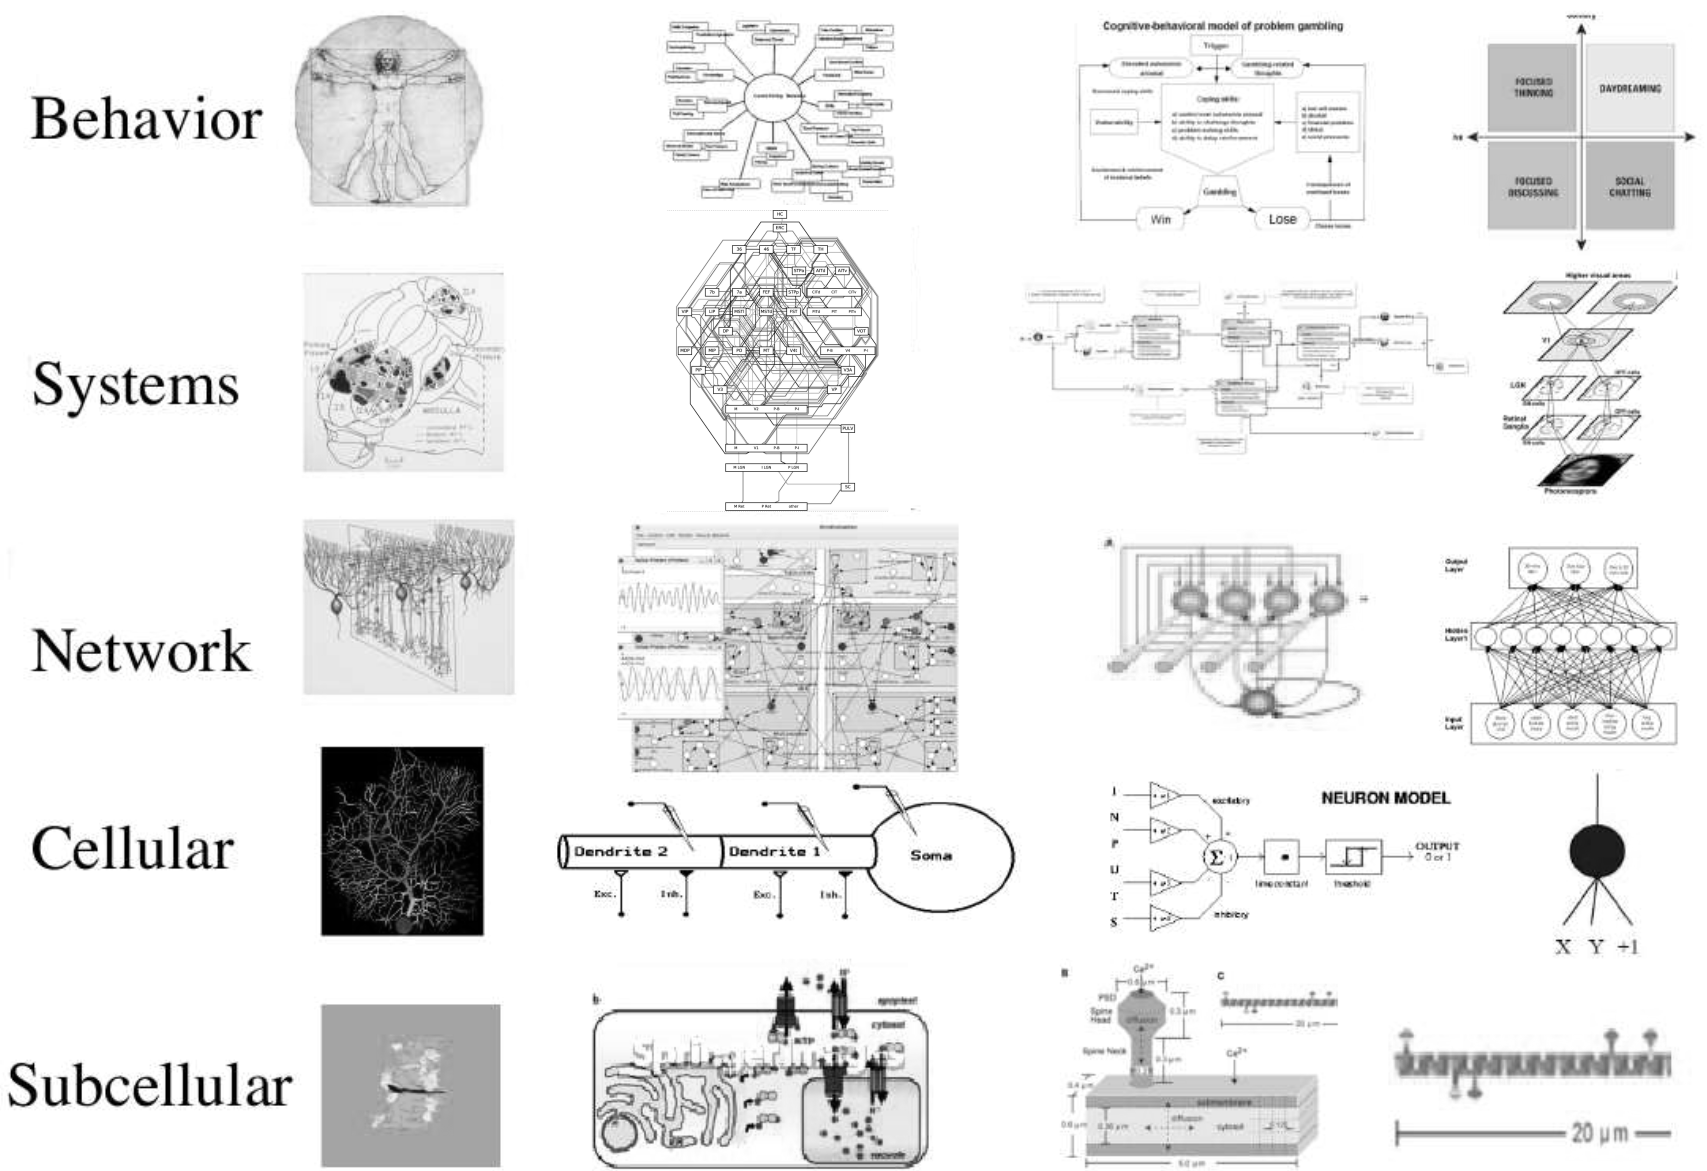
\includegraphics[width=0.9\textwidth]{figures/fig1-bw.png} %%multi-scale-taxonomy-no-arrows-no-texts.pdf}
  \end{center}
  \caption{ \small{\bf A model taxonomy.} }
  \label{fig1}
\end{figure}

Fig.\,\ref{fig1} also captures the fact that individual modeling projects within one or more laboratories typically tend to focus on the implementation and study of an individual model partitioned to a given level. This tendency acts to both isolate each research program and creates the problem of how to integrate resultant but effectively independent models. It is a problem is only exacerbated as new empirical data is acquired at any level of biological detail. In short, the matrix of Fig.\,\ref{fig1} provides a graphic illustration of what has come to be known in computational neuroscience as the multiscale problem.

As a consequence of this tendency of partitioning, it has been claimed that most simulators in computational neuroscience start out as a monolithic program~\cite{cannon07:_inter}. In this paradigm a model is defined in the same programming language as the simulator and is interwoven with a large body of code that supports simulation but is not part of the actual model. Consequently, each change of the simulation or a parameter typically requires recompilation of the entire simulator.

It has been recognized that the relationship between the biological levels is a crucial aspect of a ``total picture" as might be thought exists in Fig.~\ref{fig1}, is frequently neglected~\cite{bickle19}.  This relationship is the “glue” that binds knowledge of neuron activity to subcellular and molecular mechanisms “below” and to circuit, network, and systems activity “above." This problem is especially glaring when attempting to relate “cognitivist” psychological theories, postulating information-bearing representations and processes operating over their contents, to neuronal activities. “Co-evolution” between these explanatory levels still seems more a distant dream than an operative methodology guiding day-to-day scientific research.

By providing a useful paradigm to address multi-level concerns through computational modelling, one applied successfully in more developed physical sciences, the motivating hope was to address the interlocking levels of theory and explanation in the mind/brain through this same paradigm, to achieve comparable results~\cite{bickle19}.

\subsubsection*{Is Simulation Neuroscience the Solution?}
\label{subsection:simneuro}

In defining the field, Fan and Markram ~\cite{fan19} consider that the deep meaning of simulation neuroscience consists in reconstructing and simulating the brain from the most fundamental principles that can be isolated to understand and link the multiple layers that form the human brain (more psychologically, in their word ``ourselves''), from molecules and cells to brain function. They further note that the philosophy of simulation neuroscience originates from the will to transcend the barriers of scale and complexity during the evolution of neuronal mapping, connectivity mapping and functional mapping in the experimental and theoretical phases of brain research with the aim of giving meaning and life to data and theories.

A definition of simulation neuroscience that is more scientifically tangible, was earlier provided by Sandberg {\it{et al}.}~\cite{sandberg08}. They note that simulation mimics the outward result. However, it is one thing to extract fundamental principles to allow the multiple anatomical structures and layers that form the human brain to provide a foundation for efficient approaches to integrating disconnected datasets and knowledge that has accumulated over hundreds of years; but, as with the brain itself, it is quite a different thing to understand how such simulations should be computationally organized. In this endeavour it has become apparent that historically, the general computational approaches to simulation have typically terminated in what are referred to as intractable monolithic software architectures and the so-called multiscale problem.
%Given its thirty-five year history the second generation GENESIS simulation platforms have evolved to the point where such problems have become intractable.
This is particularly the case as despite early realization of a relation between structure and physiology~(see, for example \cite{sieck17}), there is neither a clear understanding of the relations between structure and function in the central nervous system nor a detailed understanding of their relation to behavior.

\subsubsection*{Workflows as Instigators for the Dissemination of Scientific Knowledge}

As a suggestion: General introduction to workflows required here: foundation for closed vs open workflows, relationship to publication workflows.

{\bf What about their 'incomplete' workflows?}\marginpar{\scriptsize incomplete}

\subsection*{A Brief Historical Overview: Hierarchy and Levels as the Foundation}

\subsubsection*{Evolution of the Classical Neuroscience Approach}

It is instructive to briefly review the metaphors employed as models of the mammalian central nervous system. Engulfed by the mechanical age~\cite{carlyle52}, Meyers~\cite{meyers87} gave in 1852 one answer when he proposed to his readers to imagine the human brain as a vast manufactory, in which thousands of looms, of complex and differing patterns, are habitually at work: a claim likely inspired by the mechanical world views of Descartes~\cite{descartes62} and before him Fernel~\cite{fernel67} (republished 2003). Later, it was described by Sherrington~\cite{sherrington53} as an ``enchanted loom". However, he later modified this remark by observing that: Physiology has brought us to the brain as a telephone-exchange. All the exchange consists of is switches. What we wanted really of the brain was, it would seem, the subscribers using the exchange~\cite{sherrington53}.

More recently, Lashley~(see~\cite{jorgensen21}) has warned the central nervous system can now better be understood, in the absence of mechanistic metaphors and by recognizing its essential nature, as an orchestrated constellation of cellular webs.

Since Turing's publication concerning computable numbers~\cite{turing38} and the development of the idea of the so-called, "Turing Machine," the brain as computer and processor of information has become an increasingly popular metaphor~\cite{matassi23}.

Subsequently, Simon~\cite{simon96a} has summarized the contemporary view of the structural organization of the nervous system: The hierarchical structure of biological systems is a familiar fact. Taking the cell as the building block, cells are found to be organized into tissues, tissues into organs and organs into systems. Within the cell are well-defined subsystems for example, the nucleus, cell membrane, microsomes, and mitochondria. It is such a philosophy that allows the fabrication of Fig.~\ref{fig1}.

\subsubsection*{The Hierarchy of Marr}

One hundred years after Meyers, one of the earliest practical schemes developed to provide a framework for computational modelling of neurophysiology was that developed by Marr~\cite{Marr:1982fk}. He identified three independent levels for understanding visual processing: (1) Computational theory---What is the goal of the computation, why is it appropriate and what is the logical strategy by which it can be achieved? (2) Data and algorithm---How can a given computational theory be implemented? In particular, what is the structure and content of inputs and outputs and what is the algorithm for their transformation? (3) Hardware implementation---How can structure, content and algorithm be physically realized?

An important element of this view was that higher level questions came to be considered largely independent of lower levels. Thus, analysis at the highest level, i.e. Level (1), was independent of any understanding of the algorithm(s) that supported a given computation at Level (2). Similarly, analysis at the intermediate Level (2) required no understanding concerning its physical implementation at Level (3).

One consequence of this view was emergence of a doctrine\marginpar{\scriptsize is this the 'doctrine of independence'?} that emphasised top-down as opposed to bottom-up investigation and modelling as the neurobiological facts were only a matter of implementation.

Briefly, top-down investigation relies on estimation of mean behavior at a macroscopic level; thus modeling populations, not single entities~\cite{chiacchio14}.  Alternatively, in a bottom-up approach interactions are described and followed individually. The general behavior of the system arises from the sum of the local behaviors, local activity is described with greater accuracy and approximations typical of a top-down approach are avoided.  Spatial distribution and stochastic behaviors are intrinsic features normally represented by this technique. However, as entities are followed individually, greater computational effort is required and there are no strong mathematical instruments available for analytical study~\cite{chiacchio14}.

Such schemas are typically embedded in a framework that knowingly or otherwise espouses a practice of divide and conquer where smaller and smaller parts and/or components are studied in the expectation that the whole can be understood through a divisive principle referred to as hierarchical reductionism~\cite{dawkins06}. This is despite the fact that it remains uncertain as to whether the brain can be understood as the interaction between independently describable subsystems~\cite{djurfeldt08}. Although, a recent report that started from the molecular level in a bottom-up approach that integrated molecular events into synaptic and neuronal architectures seems to provide convincing evidence that this may not actually be possible~\cite{bouteiller11}.

%Alternatively, Bojack~\cite{bojak22} has proposed that within a decade or two, top-down neural population models will take their rightful place as the primary means by which mesoscopic brain activity is described. It is claimed further that the central problem to be faced by bottom-up descriptions is not the simulation of millions of neurons in a reasonable amount of time, but rather that the properties and interactions of that number of neurons cannot be specified in a biologically meaningful manner and cannot generate actual human insight into principles of function from the plethora of individual cell activities. Rather, progress is to be made via multiscale descriptions wherein higher levels discard the irrelevant detail of lower levels to facilitate effective and efficient models that remain accessible to the human mind. Further, it is expected that in the future, given their intimate connection to (noninvasive) neuroimaging, such neural population models will play a privileged role.

% Thus, for the foregoing reasons, amongst others canvassed here, the metaphors employed to provide the framework for the cognitive models subserving neuroscience in general and computational neuroscience in particular, must be chosen with great care.

% Ultimately, however, computational neuroscience is proposed to offer multiscale models that span complexity from the level of the gene to the whole living system, spanning different temporal and spatial scales~\cite{jung22}.

\subsubsection*{The Hierarchy of Churchland and Sejnowski}

More recently, Churchland and Sejnowski (1992) (C\&S)~\cite{Churchland:1992uq} proposed a seemingly more sophisticated version of Marr's three level schema~\cite{Marr:1982fk}: (1) Level of analysis, which includes Marr’s three levels, (2) Level of processing, for example the levels of processing in the visual pathway and (3) Level of structural organization, for which they proposed seven general levels (Systems, Topographic Maps, Layers and Columns, Local Networks, Neurons, Synapses, Molecules)~\cite{Churchland:1992uq}.  In developing their perspective, a number of fundamental observations were made.

Importantly, it was noted that the doctrine of independence\marginpar{\scriptsize 'doctrine of independence' should be explained more / defined first} confuses two very different issues. One concerns whether as a matter of discovery the relevant algorithm can be determined, while the other concerns whether as a matter of formal theory, a given algorithm already known to perform a task on a given machine (in this case, the brain) can be implemented on a machine with a different architecture. Computation theory suggests that if an algorithm is independent of its implementation it can be implemented on different machines with different architectures as none of the requisite physical parameters are part of the algorithm. In short, however, there is no formal theory to confirm whether the discovery of the algorithms relative to cognitive function are independent of the detailed structure of the nervous system.

As has already been suggested above, in contrast to the doctrine of independence, current research appears to confirm that implementational considerations play a vital role in the kinds of algorithms that tend to be devised and the types of computational insights that they provide (C\&S). Further, knowledge of brain architecture, far from being irrelevant as assumed by top-down models, may provide an essential basis for likely and powerful algorithms.

\subsection*{Is Hierarchy a Good Foundation?}

% \subsubsection*{Contrasting the Classical Approaches with the Observations}

% One of the most surprising statements associated with the emergence of computational neuroscience was made by C\&S. As suggested by Figure\,\ref{fig2}, they postulated the primacy of levels as a foundation of the computationally modern view of the neurobiological research paradigm. Given the historical and scientific considerations referred to above, such a dogmatic stance appeared to be a reactionary curiosity, even when initially proposed. An important question then becomes, how was such an assumption so central to understanding the neural structures and functions that subserve neurophysiology?

% One explanation of C\&S's position on levels is as a simplifying statement that greatly increases the tractability of gaining better understanding of the mammalian central nervous system. This is despite going against powerful observational and theoretical evidence that seems to support a novel emerging understanding of the highly dynamic structure and function of the human brain. A significant initiating contribution to that newly evolving understanding may be found in observations made by anatomists such as Bell~\cite{bell11}.  More than 200 years ago, he noted that in the lack of any consistent history of the brain and nerves\marginpar{\scriptsize history of the brain and nerves???}, along with the dull unmeaning manner of demonstrating the brain, any novelty in the manner of treating the subject was authorised. Further, that it is no more presumptuous to follow the tracts of nervous matter in the brain and attempt to discover the course of sensations, than it is to trace the rays of light through the humours of the eye and to say that the retina is the seat of vision.

% Comments such as those made by Bell~\cite{bell11} are supported by observations made more than 250 years previously by Fernel and followed a century later by Descartes who was impressed by the hydraulic figures in the royal gardens at Saint-Germain-en-Laye and developed a hydraulic theory of the action of the brain~\cite{cobb60}. In the {\it{Treatise on Man}} Descartes supposes~\cite{descartes04a}: The body to be just a statue or a machine \ldots which God forms with the explicit intention of making it as much as possible like us. He goes on to leaven this supposition by further supposes that: This machine is made by God and he thinks that the reader will agree that the body is capable of a greater variety of movements than he could possibly imagine in it and that it exhibits a greater ingenuity than he could possibly ascribe to it. In so writing, Descartes ~\cite{descartes04a} (although according to Sherrington~\cite{sherrington53} he was putatively following Fernel~\cite{fernel67}) is considered to have originated the view that living organisms worked as machines and insisted on a class of motor acts, animal and human, in which the thinking soul takes little or no part~\cite{descartes62}.

\begin{figure*}[h!t]
  \begin{center}
  \vfill{}
    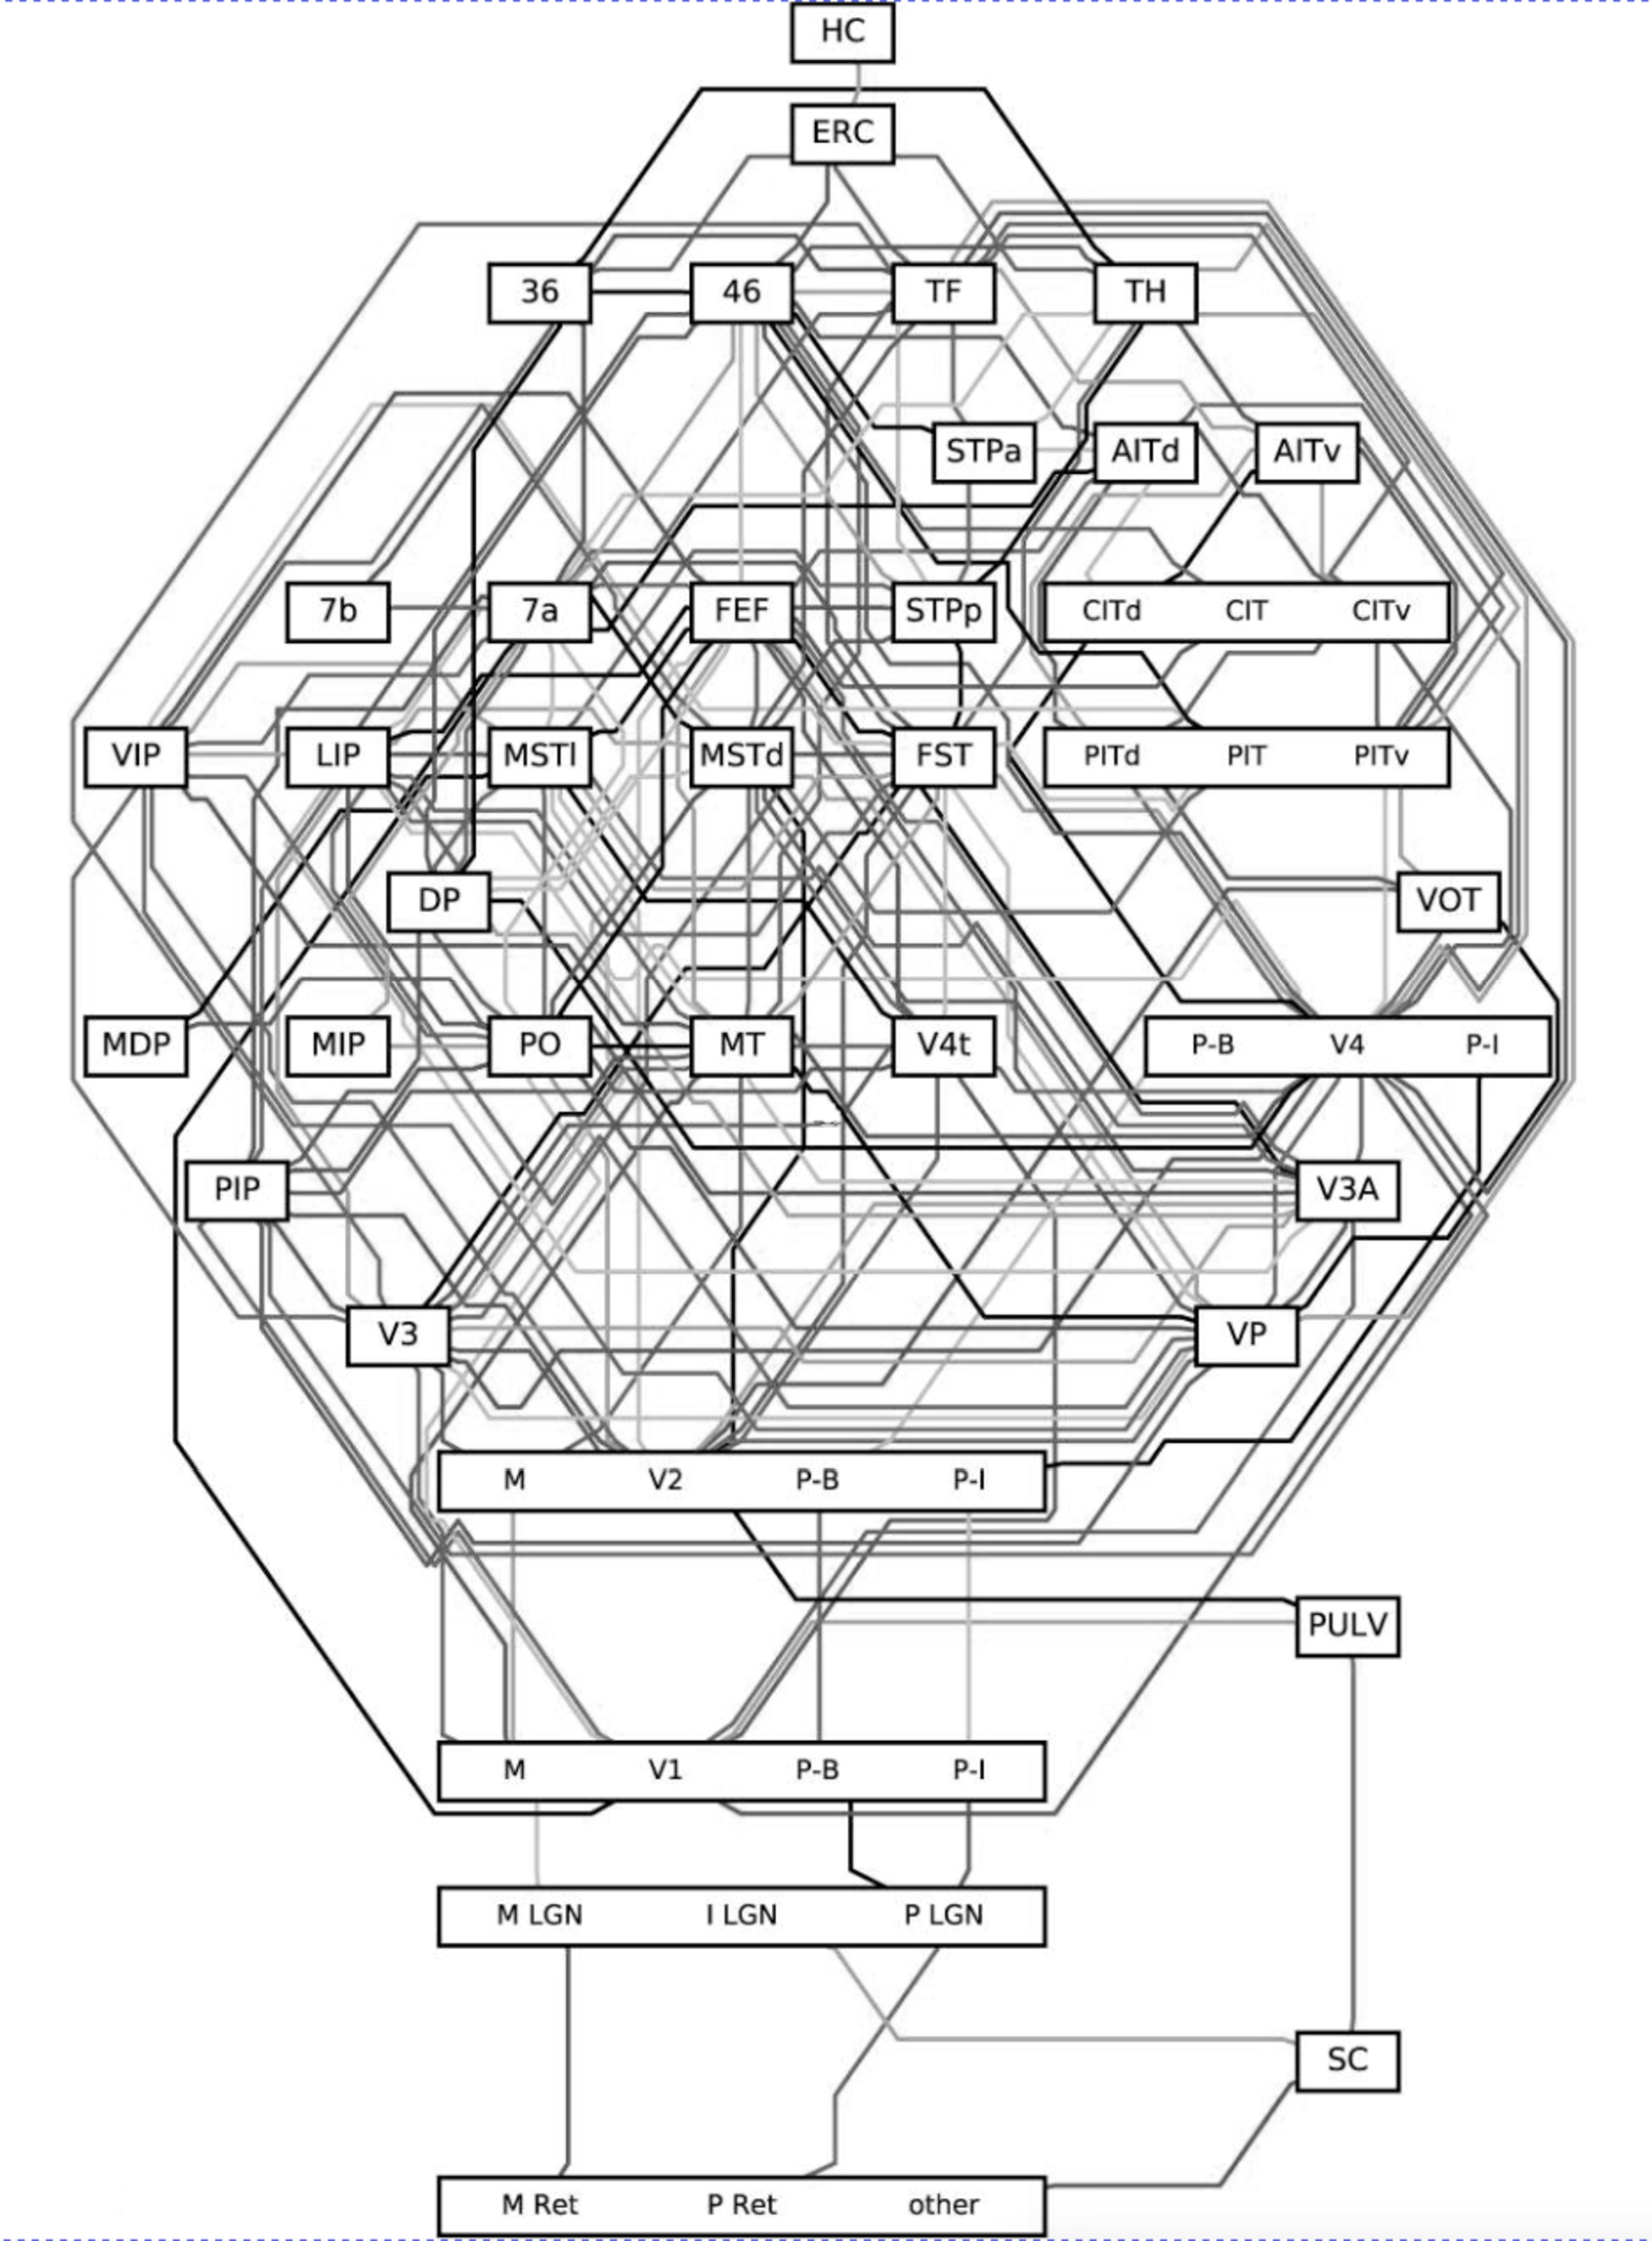
\includegraphics[width=0.45\textwidth]{figures/van-essen-primate-vision-circuit-grayscale.pdf}
  %\vfill{}
    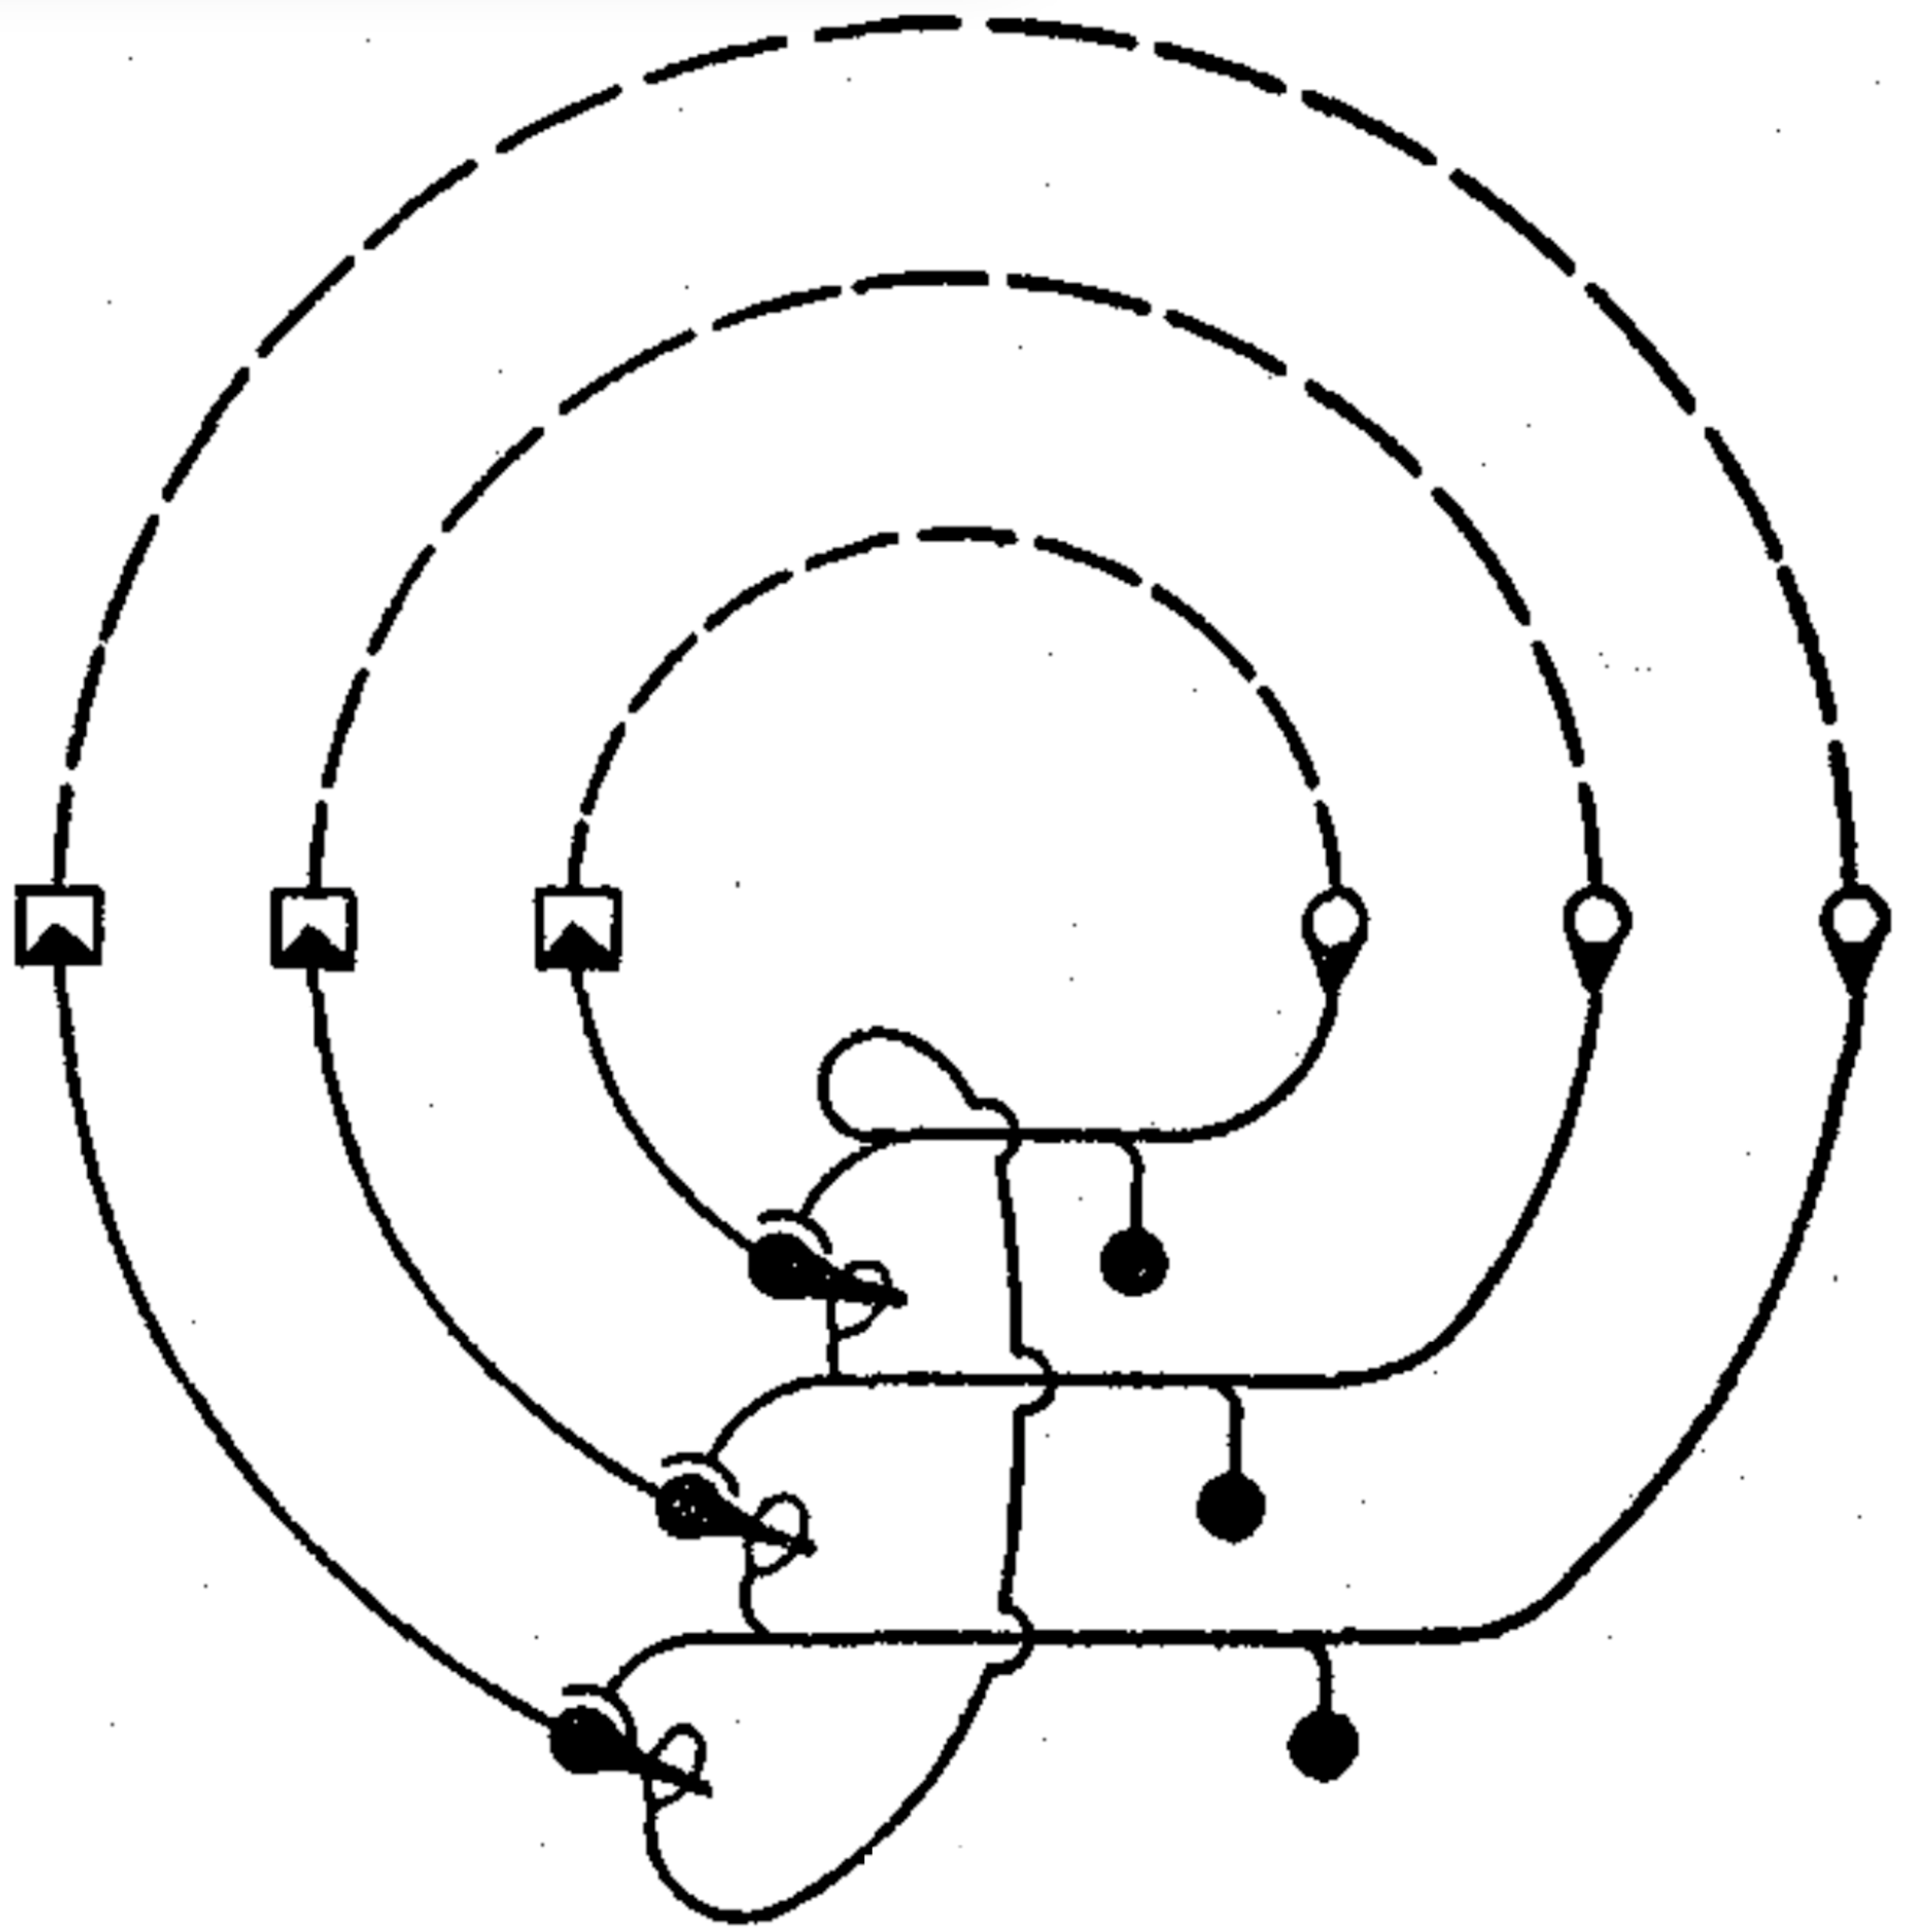
\includegraphics[width=0.45\textwidth]{figures/mcclelland-heterarchical-circuit.pdf}
  \end{center}
  \caption{{\bf Are the results of observations really hierarchical?}  \small{\bf{Left:}} A proposed hierarchical structure of the visual system.  Here, it is proposed that on the basis of panel (A), if it is assumed that in the given illustration of circuits underlying primate visual processing the labels in this panel are hierarchically arranged it might not be surprising that progress may be slow, (see~\cite{jonas17} for details). Such an interpretation is supported by Cobb ~\cite{cobb60} that: It should be a fundamental principle of neural interpretation of psychological functions are that the nervous activities are as complex as the psychological activities that they constitute.
    {\bf{Right:}} Circularities, instead of indicating inconsistencies, actually demonstrate heterarchical consistency of a higher order than is possible with a hierarchical approach. Further, an organism possessed of a nervous system arranged in the illustrated way, but possessed of double the number (six) of neurons, would be unpredictable for any hierarchically structured theory (see~\cite{mcculloch45a} for details).
    (Left panel adapted from~\cite{fraser21} Fig.\,1B).}
  \label{fig2}
\end{figure*}

\subsubsection*{The Heterarchy of Values}

As Bell noted~\cite{bell11}, things appear sufficiently simple and consistent until the structure of the brain and the course of the nerves are begun to be examined anatomically. Then all is confusion. The divisions and subdivisions of the brain, the circuitous course of nerves, their intricate connections, their separation and reunion, are puzzling in the last degree and are indeed considered as things inscrutable. Thus, those who know the parts the best are the most in a maze. While, those who know the least anatomy, see the least inconsistency in the commonly received opinion. In short, functional and structural brain connectivity matters (see, for example,~\cite{gili18}).

By the middle of the twentieth century it could be seen that the classical hierarchical viewpoint of brain structure and function comprised of levels associated with different physical scales was beginning to be upended by theoretical publications such as that authored by McCulloch~\cite{mcculloch45a}. Entitled, {\it{A heterarchy of values determined by the topology of nervous nets}}, it proposed that because of both the reciprocal nature of purposive activity, the closed circuits that sustained it and their interaction, the circuits can be treated topologically. If it is recognised that {\it{A}} is preferable to {\it{B}}, {\it{B}} to {\it{C}}, but {\it{C}} is preferred to {\it{A}}, there is a  corresponding circularity in the net that is not the path of any one circuit and cannot be mapped as such (see Fig.~\ref{fig2}).

McCulloch~\cite{mcculloch45a} concluded that an organism possessed of such a nervous system---six neurons--- is sufficiently endowed to be unpredictable from any theory founded on a scale of values. It lacks a hierarchy of values and instead exhibits a heterarchy of values and thus its connectivity is too rich to submit to a {\it{summum bonum}}.

A subsequent letter to the editor further clarified aspects of the publication by elaborating that: {\it{A}}, {\it{B}} and {\it{C}}--so connected that no one sustains activity without summation from the afferent component of one other projection and letting the net be such that {\it{B}} (and only {\it{B}}) necessarily contributes to {\it{A}} ; similarly, {\it{C}} (and only {\it{C}}) to {\it{B}} and {\it{A}} (and only {\it{A}}) to {\it{C}}. Presented with a stimulus {\it{a}}, {\it{b}}, or {\it{c}} separately, there will be no response; but given any pair, {\it{a}} and {\it{b}}, or {\it{b}} and {\it{c}}, or {\it{c}} and {\it{a}}, the organism will appropriate {\it{a}}, {\it{b}}, or {\it{c}}, respectively; and given {\it{a}}, {\it{b}} and {\it{c}}, the organism will appropriate all three. Obviously, this net resembles Figure~4 in~\cite{mcculloch45a} (here given for convenience in Fig.~\ref{fig2}\,Right) and the same topological considerations apply, except that in the current case the threshold of the afferent neurons is now such as to require impulses from the terminations of two axons and that the different excitatory fiber actions sum instead of inhibit as in the previous example. The preference, whether or not it be a true choice, is determined by a pair of projections, which is no less an activating combination of fibers because the differential connectivities of the projections sum instead of inhibit~\cite{mcculloch45b}. To summarize, in neither case is the activity of such a circuit hierarchical in nature.

It is currently believed that a successful study of phenomena across a wide range of scales requires various cognitive resolutions of abstraction. These abstractions are considered to range from precise biophysical interactions to the functions they implement. To introduce a widely promulgated view of the subject, it has been argued that neuroscientific practice is facilitated within a pragmatic perspective whereby descriptive, mechanistic, and normative models and theories each play a distinct role in defining and bridging these levels of abstraction. In short, these labels correspond to three different explanatory approaches in neuroscience, which are used to respectively solve three different types of problem: “what” problems, “how” problems, and “why” problems~\cite{dayan01}. Such analysis is proposed to lead to methodological suggestions, including selection of the level of abstraction deemed appropriate for a given problem, identifying transfer functions that connect data to models, and the employment of models as a form of experiment~\cite{levenstein23}.

On the basis of technological advances, new experimental approaches and subfields have generated rapid growth and revealed a pressing need for the development of new theoretical frameworks (but see~\cite{phillips15}). However, despite the fact that some of the greatest successes in neuroscience have been reliant on well publicised mixtures of theory and empiricism (see for example,~\cite{hodgkin52e,okeefe78,traub91,marr10,vaina91}), disagreement remains about the nature of theory and its role in neuroscience, including how it should be developed, used, and evaluated~\cite{bialek18,goldstein18}. Nevertheless, because the phenomena of interest are conceived of as spanning a wide range of spatiotemporal scales, it is believed their explanation requires a “multilevel” approach that combines data from quite different modalities~\cite{levenstein23}.

As suggested above, three different types of explanation are considered to each play a distinct role in the building of a multilevel account of neural phenomena. Descriptive explanations provide an abstract characterization of a phenomenon, while mechanistic and normative explanations bridge abstractions of different levels. Collectively, these operations are proposed to unify scientific theories across disparate experimental approaches and fields. It is a view considered to facilitate the bidirectional interaction between theory and experimentation as well as theory development itself~\cite{levenstein23}.

According to this pragmatic view, progress results from community maintained standards of explanation driven by an urge to better predict and control natural phenomena of potential relevance to society. Thus, by shifting theories from “proposals of truth to be falsified” to “proposed problem-solving tools,” the pragmatic view prompts assessment of a theory by its utility: what empirical problems it can solve, how easily it can be used to solve them, and how good its solutions are. Through competition to solve empirical problems, theories become more precise, provide clearer and more concise explanations, can be used to make more reliable and accurate predictions, and can be applied to larger domains (see~\cite{levenstein23} and~\cite{douglas14} for further detail). 

\subsubsection*{Contrasting the Classical Workflows with the Processes for Increasing Scientific Knowledge}

Proposed section that contrasts the workflows proposed by Markram with the workflows that are required to 'close the loop'.

This may also hint at the need for better methodology for publications for modeling in Neuroscience.

%% "On several occasions, I presented such views (Nadin 2000, 2003, 2009b, for example), informed by Rosen’s work and by other attempts to free science from a limiting view of how knowledge is acquired."

%% Not just, how is knowledge acquired and how do the methods interact with what is acquired, but also how is knowledge communicated and how does the communication method interact with the communication.

\subsection*{A Different type of Neuroscience: Emulation Neuroscience}
\label{subsection:emuneuro}

%%\marginpar{\scriptsize The scheduler and the model-container are both scale- and level-independent / -agnostic.  The model-container supports 3D multi-resolution models consisting of polygons, traditional neuroscience multiscale models and, when needed / required, heterarchical models.  In 3D polygon models the parameterization of the model defines its spatial scale of resolution, in typical neuroscience models, the used entities such as neurons and networks, define the spatial scale of resolution. }

The term emulation originates in computer science, where it denotes mimicking the function of a program or computer hardware by having its low-level functions simulated by another program. An emulation is regarded as successful if the emulated system produces the same outward behaviour and results as the original (possibly with a speed difference). This is a somewhat softer requirement than that of a strict mathematical definition~(see, for example \cite{sandberg08}).

% Thus, as mentioned above, if brain activity is regarded as a function that is physically computed by brains, then it should be possible to compute it. Even if true, however, it does not demonstrate that it is a computationally feasible process~\cite{sandberg08}.

Here, in contrast to a simulation which computes a model where only some properties exist, an emulation refers to a one-to-one model where all relevant properties of a system exist~\cite{sandberg08}. Further, it is noted that although emulations may behave differently from each other or the original due to noise or intrinsic chaos, they should still behave within a range that might be expected from the original if it had been subject to the same interference.

As such, emulation neuroscience is a pragmatic discipline that allows to compute heterarchical structures as is required for the animate, founded on fact rather than subservience to authoritative historical belief.  Further, that, the means by which emulation neuroscience may progress knowledge, especially scientific knowledge, as Popper has noted~\cite{popper62}, does not preclude unjustified (and unjustifiable) anticipations, by guesses, by tentative solutions to problems, by conjectures. Conjectures that are controlled by criticism; that is, by attempted refutations, which includes severely critical tests. although they may survive the tests; they can never be positively justified: neither can they be established as certainly true nor even as `probable' (in the sense of the probability calculus).

\subsubsection*{What is Scientific?}
In part because the historical understanding of science was independent of a stipulated method for obtaining answers to ``why" questions and especially because it did not focus on empirical or observational procedures, that older and more comprehensive understanding of science has slowly been eroded since the Enlightenment. The view that science is content-determined in terms of the kinds of questions it must answer, has been replaced by method-based procedures. Thus, something is scientific on the basis of how it was obtained, not by what it is about. This is a massive shift in outlook and as a result the question as to what is ``scientific knowledge" shifts from the semantic to one of ``scientific method." Consequently, the limits of scientific knowledge have shifted from something that is content-based to something quite different: the adequacy of an admissible methodology. These two understandings of science are incommensurate with the worst feature being that there is no real consensus as to what methods are to be allowed as unquestionably producing scientific knowledge.

It therefore seems both reasonable and timely to propose that, evolution of the classical foundational fields of computational and simulation neuroscience~(see, for example~\cite{fan19,swanson15,swanson10}) is drawing to a close. Absent such extinction, what remains is only an increasingly unsustainable oxymoron, one firmly ensconced in a seemingly perpetual theo-philosophical and increasingly mechanistic world view. However, by its transcendence, a greater veracity and human understanding can be infused into both the cognitive models that remain to both be fabricated and implemented and their increasingly seamless juxtaposition with the neurobiology they purport to explain. %%emulate.

\section*{Materials and methods}

% Similarly, from the viewpoint of software architecture it has been found extremely complicated to integrate the software systems that implement these isolated independent models.  In software engineering literature such a problem is referred to as the monolithic problem [citation needed?].
%In the 1970s and 1980s, with the advent of personal computers and the rise of client-server architectures, the focus shifted towards more distributed systems. Monolithic architectures persisted, with many large software applications, such as enterprise resource planning (ERP) systems, continuing to rely on a centralized architecture.
% This problem typically manifests after continual modification and/or expansion of a software platform.  It results in coding systems that have become increasingly unmanageable.

\subsection*{Simulators as a Tool for Embedding Workflows}
Two notable exceptions that attempted to address the problems associated with multi-scale modeling have been the GENESIS-2 and NEURON simulators.  The architecture of GENESIS-2 facilitated an object-oriented programming environment where independent objects in the simulator represented biological concepts in the real world. This greatly facilitated parallel development and extension, with the further important advantage that it allowed easy parallelization of simulations~\cite{goddard97:_paral_genes}. However, a significant problem was the consequent match of biological concepts with their mathematical implementation. This created a simulator that exposed considerable technical detail to the user and ultimately gave rise to increased investigator befuddlement concerning model development.

As was noted above, realistic neural software platforms such as GENESIS-2 and NEURON were not immune to the latter software ``feature." It might further be noted that GENESIS employed a fully, ``collaborative development model"~\cite{gewaltig14} from its initial public release (1990), whereas it took a further 32 years for NEURON to emerge from a, ``heroic development model"~\cite{gewaltig14}. In fact,
% similar to how the GENESIS-2 Modeler's Workspace initiated NeuroML development~\cite{nigel01:_towar_neurom},
% the reconfiguration of the software architecture of GENESIS 2.4 that evolved GENESIS-3~\cite{cornelis08:_cbi_archit_comput_simul_realis,cornelis08:_model_neuros_genes} preceded the recent radically updated development model, life cycle, workflows, code checking and documentation of the NEURON software (Version 8.1)~\cite{awile22} by some 15 years.

% The history of monolithic architectures can be traced back to the early days of software development, with the emergence of large mainframe computers in the 1950s and 1960s. These early computer systems were characterized by a centralized architecture, with a single mainframe computer serving as the hub for all computing operations.

% Although the GENESIS simulator initially avoided such problems, with continued development of the software associated with computational models and their simulation, the simulator incrementally became monolithic as it acquired increased scale and complexity. 

In this section, an alternative approach is introduced that includes a brief historical review and description of the principles and components of scientific and user workflows developed to support flexible arrangements of model taxonomies as exemplified in Figure\,\ref{fig1}; along with some of the abstract paths that can be employed to reduce the exigent problems that have arisen from the discrepancy between cognitive models and the effective computational emulation of reality. The achievement is the fabrication of a dynamic generalized framework and resultant emulator architecture that leads to descriptions and illustrations of a fully implemented, scale-independent software platform, G-3/Neurospaces.

\subsection*{So, What Is Scientific?}

When initiating a new project it is often of value to explore the meaning and origins of the semantics within which it is buried. Here, the interest lies in elucidation of a framework that enables what is referred to as scale-independent neural emulation.

For more than 1,500 years anatomical and physical ideas concerning the structure and function of the human nervous system settled into an enduring dogma that encompassed the time of Galen ({\small{AD}}\,129--199) in antiquity to that of Haller ({\small{AD}}\,1708--1777) in the eighteenth century~\cite{clarke87}. It subsequently disappeared during the first half of the nineteenth century as a scientific revolution ushered in a new understanding of the nervous system. Outmoded ideas were displaced by fundamental new neuroscientific concepts of the nervous system that were developed, became established during that half century and subsequently have survived in modified form into the twenty-first century. In short, it is not unreasonable to consider that by 1850, with the exception of the idea of localization of function in the brain, the foundations of modern experimental neuroscience had been laid.

Deeply influenced by a long enduring world view, the philosophical thought of that time became embedded deep within an otherwise inexplicable change in the experimentalist's attitude to brain activity that could be attributed to investigators such as Flourens on the basis of his claim that in experimental research everything depends on the method~\cite{flourens24}.

Technology, however sophisticated, is only one element of scientific creativity. The human element in science is primary. An investigator must frame meaningful questions, devise programs of research and draw productive conclusions if there is to be any significant contribution to knowledge~\cite{clarke87}. Nowhere is this likely better demonstrated than with the identification of electricity with nervous activity by Galvani (1770)~\cite{galvani91} when he demonstrated muscle contraction in the frog leg after a wire in contact with a nerve fibre conducted an electrical spark. It then took almost 200 years via Nernst~\cite{nernst89} and Lapicque~\cite{lapicque07} before Hodgkin and Huxley~\cite{hodgkin52e} mathematically described the differential conductances in the membrane of a squid nerve fibre that underlay the generation of an action potential. It was with those experiments and their mathematical model that computational neuroscience came of age.

In one important way, many predictions in the biological sciences differ from those made in the physical sciences, particularly classical physics~\cite{darwin71}. In physics and engineering, most simple predictions or tests of hypotheses are deterministic. Whereas, in biology and particularly in neuroscience, many predictions where they can be made, are inherently probabilistic, thus not as much deterministically causal as unpredictably relational.

In this section, the constraints of the various cognitive models that led to the CBI Federated Software Architecture (for details, see \cite{cornelis12,cornelis08:_cbi_archit_comput_simul_realis}) are illustrated and briefly reviewed. These include: Data flows for computational implementation of cognitive models (see Fig~\ref{fig2}), an ideal user workflow (see Fig~\ref{fig3}), and examples of different cognitive paths from mental models to simulation at different spatial resolutions (see Fig~\ref{fig4}).
%%, a relational diagram of the four fundamental components resulting from a principal concerns analysis (see Fig~\ref{fig6}) and an overview (see Fig~\ref{fig7}) and detailed view (see Fig~\ref{fig8}) of the Computational Biology Initiative Federated Software Architecture that organizes the reconfigured GENESIS (G-3).

\subsection*{What is Common: Workflows and the Scientific Process}

\subsubsection*{The Scientific Workflow Paradigm}

The relationships between the activities involved in conducting an experiment and running a simulation are illustrated in Figure\,\ref{fig3}.  This figure illustrates two iterative processes connected by a feedback loop that employs interpretation of results as an iterator to design new experimental setups and model constructions.

\begin{figure}[h!t]
  \begin{center}
    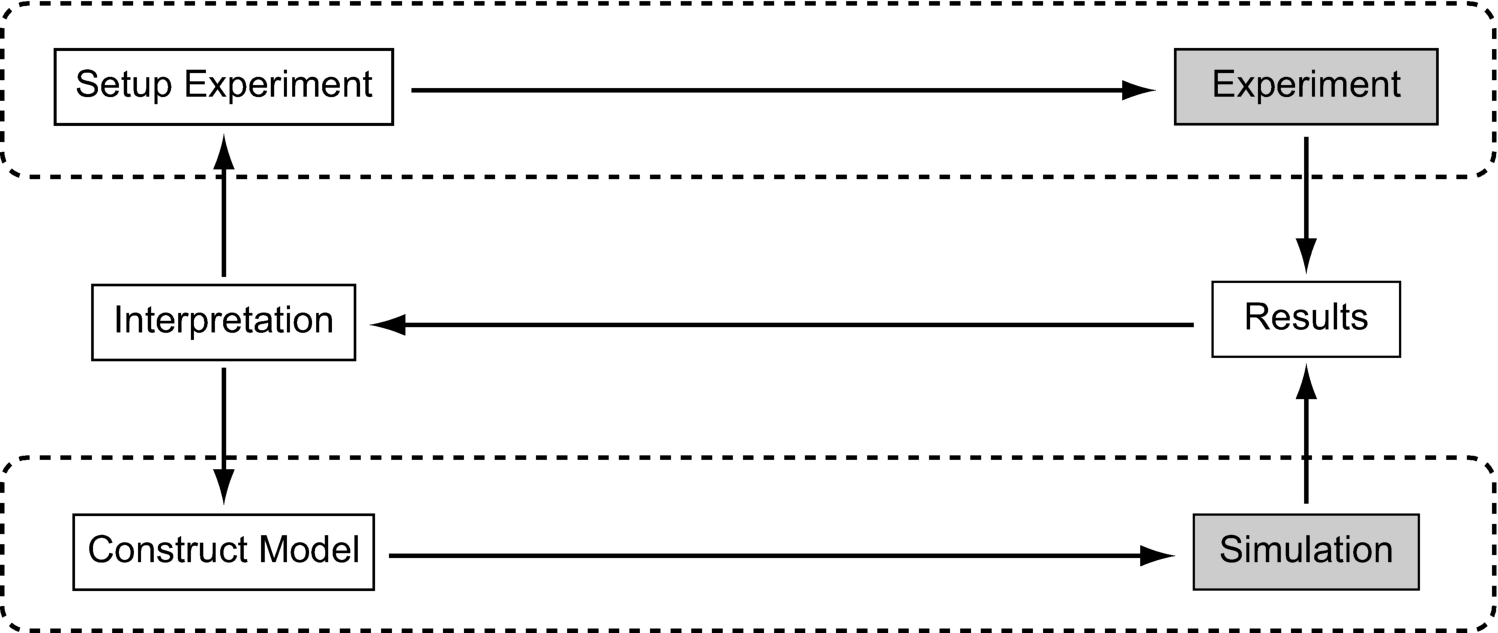
\includegraphics[width=0.75\textwidth]{figures/exp-sim.pdf}
  \end{center}
  \caption{ \small{\textbf{Data flows in science}. Conducting experiments and running simulations are part of two processes delineated by the upper and lower dashed outlines. They are connected by an interposed feedback loop that uses iterative interpretation of results to design new experimental setups and model constructs.}}
    \label{fig3}
\end{figure}

From this perspective, simulation provides a framework to organize the understanding of biological systems. The software architecture introduced here (described in following subsections) is designed to support the lower loop within Figure\,\ref{fig3}. It was developed to resolve the complexities associated with continual addition of functionality to a simulator. To reiterate, historically, simulators have become monolithic and it has become increasingly difficult for users and developers to maintain and extend them. The logical consequence is that user workflows are often similarly degraded. One consequence is that contemporary simulator scripts are typically unstructured in the sense that a biological model is mixed with other code that defines and controls inputs, outputs and simulation configuration~\cite{cannon07:_inter}.

Importantly\marginpar{\scriptsize new paragraph} the iterator step of 'interpretation' of results provides the necessary step for communication among scientists and thus for scientific publications.  As such, scientific publications close the loop of scientific knowledge production.  From a computational modeling perspective for the animate world this comes with the consequence that the publication systems employed in the biological science have fundamentally different requirements when compared to the publication systems for the physical sciences of the inanimate world.

\subsubsection*{Application of the Workflow Paradigm to Neuroscience}

In response to these circumstances, in an effort to avoid the bureaucratic overthink of ``mega-projects" by bypassing the epistemological and methodological metaphors often associated with the workflows of such juggernaut brain research~\cite{fan19}, a five step “ideal user workflow”, or user workflow has recently been proposed~\cite{cornelis12}.

\begin{figure}[h!t]
  \begin{center}
    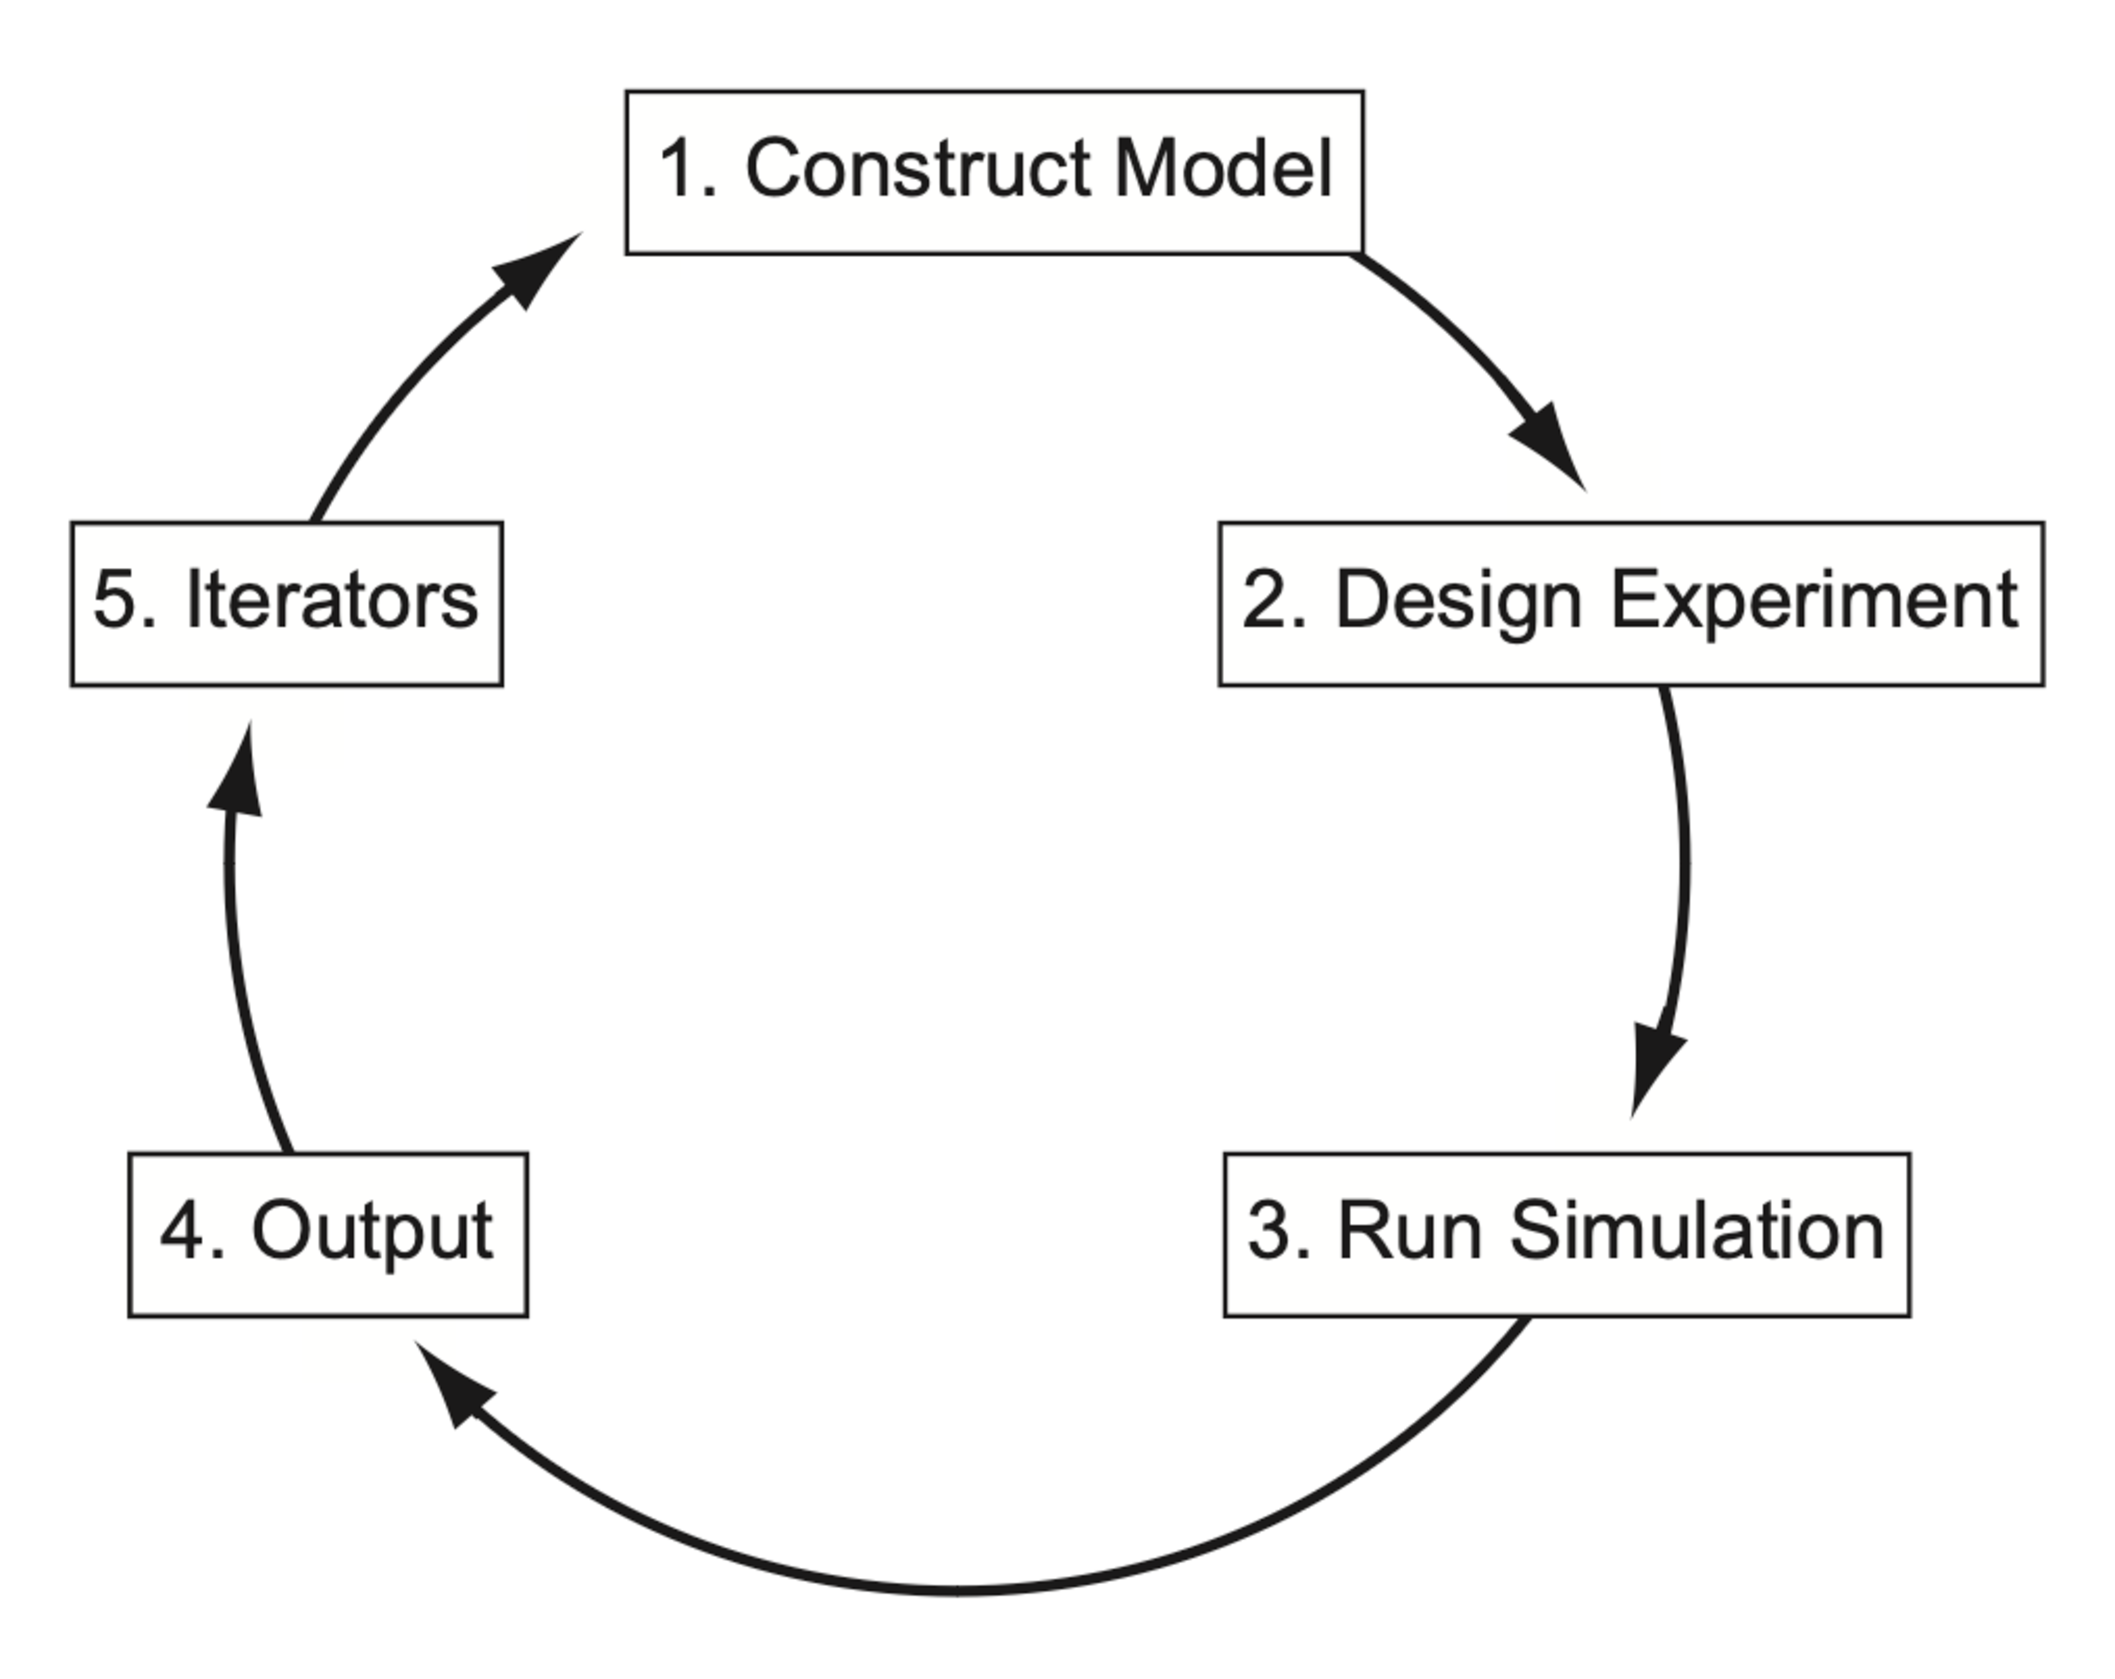
\includegraphics[width=0.50\textwidth]{figures/user-workflow.pdf}
  \end{center}
  \vspace*{-\lineskip}
  \caption{ \small{{\bf The five steps of the ideal user workflow.} {\textbf{1.\,Construct Model:} Simple models can be created directly within the GENESIS$^*$\,\textit{G-Shell} by entering commands. More complex models can be imported into the\,\textit{G-Shell} from either the GENESIS model libraries or from external model libraries. The model can also be explored, checked and saved. Changes made to the components of a model during a research project include changes to connectivity, cell morphology (e.g. spines) and membrane conductances. \textbf{2.\,Design Experiment:} Set model parameter values specific to a given simulation, the stimulus parameters for a given simulation run or 'experiment' and/or the variables to be stored for subsequent analysis.} \textbf{3.\,Run Simulation:} Configure runtime options, check, run, reset simulation and save model state. The model state can be saved at any simulation time step to allow it to be imported into a subsequent GENESIS session. Output is flushed to raw result storage for subsequent data analysis. \textbf{4.\,Output:} Check simulation output and the validity of results to determine whether simulation output exists in the correct locations. Output can be analyzed either within GENESIS or piped to external applications such as Matlab, Grace, or Mathematica. \textbf{5.\,Iterators:} Close the loop between output of results and model construction in the GENESIS users workflow. Iterators connect experimental results and model output and include for example, automated construction of simulations and batch files, static parameter searching and active parameter searching using the dynamic clamp. $^*$\,Version 3.0.}}
  \label{fig4}
\end{figure}
%\FloatBarrier

This workflow (see Figure\,\ref{fig4}) organizes the sequence of activities typically employed for the development and simulation of a computational model, including data generation and analysis.  It consists of five steps: 1.\,Construct model, 2.\,Design experiment, 3.\,Run simulation, 4.\,Analyze output and 5.\,Iterate.  Such a workflow allows the model under investigation, the tools used to perform the investigation and the operations performed during a simulation to be distinguished. These categories correspond to the approaches to computational modelling previously identified by Marr.

%% For clarification, in the biological domain we refer to ‘multi-level’ (level), in the modelling domain we refer to ‘multiscale’ (scale) and in the software domain we refer to ‘multi-layer’ (layer).
%%\FloatBarrier %% will force figure to specified location
Here, the workflow paradigm is extended by introduction of an organizing principle, the “cognitive workflow”. This workflow describes the process whereby a cognitive abstraction is transformed into an implementation by the conversion of a mental model into a physically instantiated simulation. In doing so, the characteristic labels that historically have come to be associated with descriptions of the classical approach to neurobiological computational simulation have been modified. This important evolutionary step aims to avoid the imposition of interpretations onto the putative structure, contents and functions of neural tissue. In other words, the aim is to minimize the teleology of an explanatory computational model devolving into a merely descriptive demonstration model.

To this end, each step in a given cognitive workflow can be expanded into a matrix where columns span the range of structural detail available at a given resolution of simulation.  As one example of such a workflow, here \ldots  The other steps in the cognitive workflow can similarly be expanded to collectively give a comprehensive framework for scale-independent modelling.

If it is accepted that: (1) a scale-independent approximation can be abstracted at each resolution of a system and disjointly partitioned from its environment~\cite{Bertalanffy:1973zr, Heylighen:2006vn} and (2) the biological domains implied by Figure\,\ref{fig1} are plausible, then it is apparent that even a realistic neuron model comprised of at least a soma and dendrites, that includes channels and synapses, is a model simulated at multiple resolutions.

Thus, one example of a cognitive workflow that facilitates such a path from the cognitive to the physical is given by the top row in Figure\,\ref{fig5} (Biology \textrightarrow\,\,Computer Science).  In this figure, the column to the left gives domains of interest (where the domain identifies the object or event under investigation) and lists domains of biological organization, the column to the right lists the equivalent domains of the software and hardware (operations performed during the investigation) and the central columns give the nature of the mathematical implementation or algorithm (tools used to perform the investigation).  The column items in each row give examples of possible simulator functionality.

\begin{figure}[h!t]
  \begin{center}
    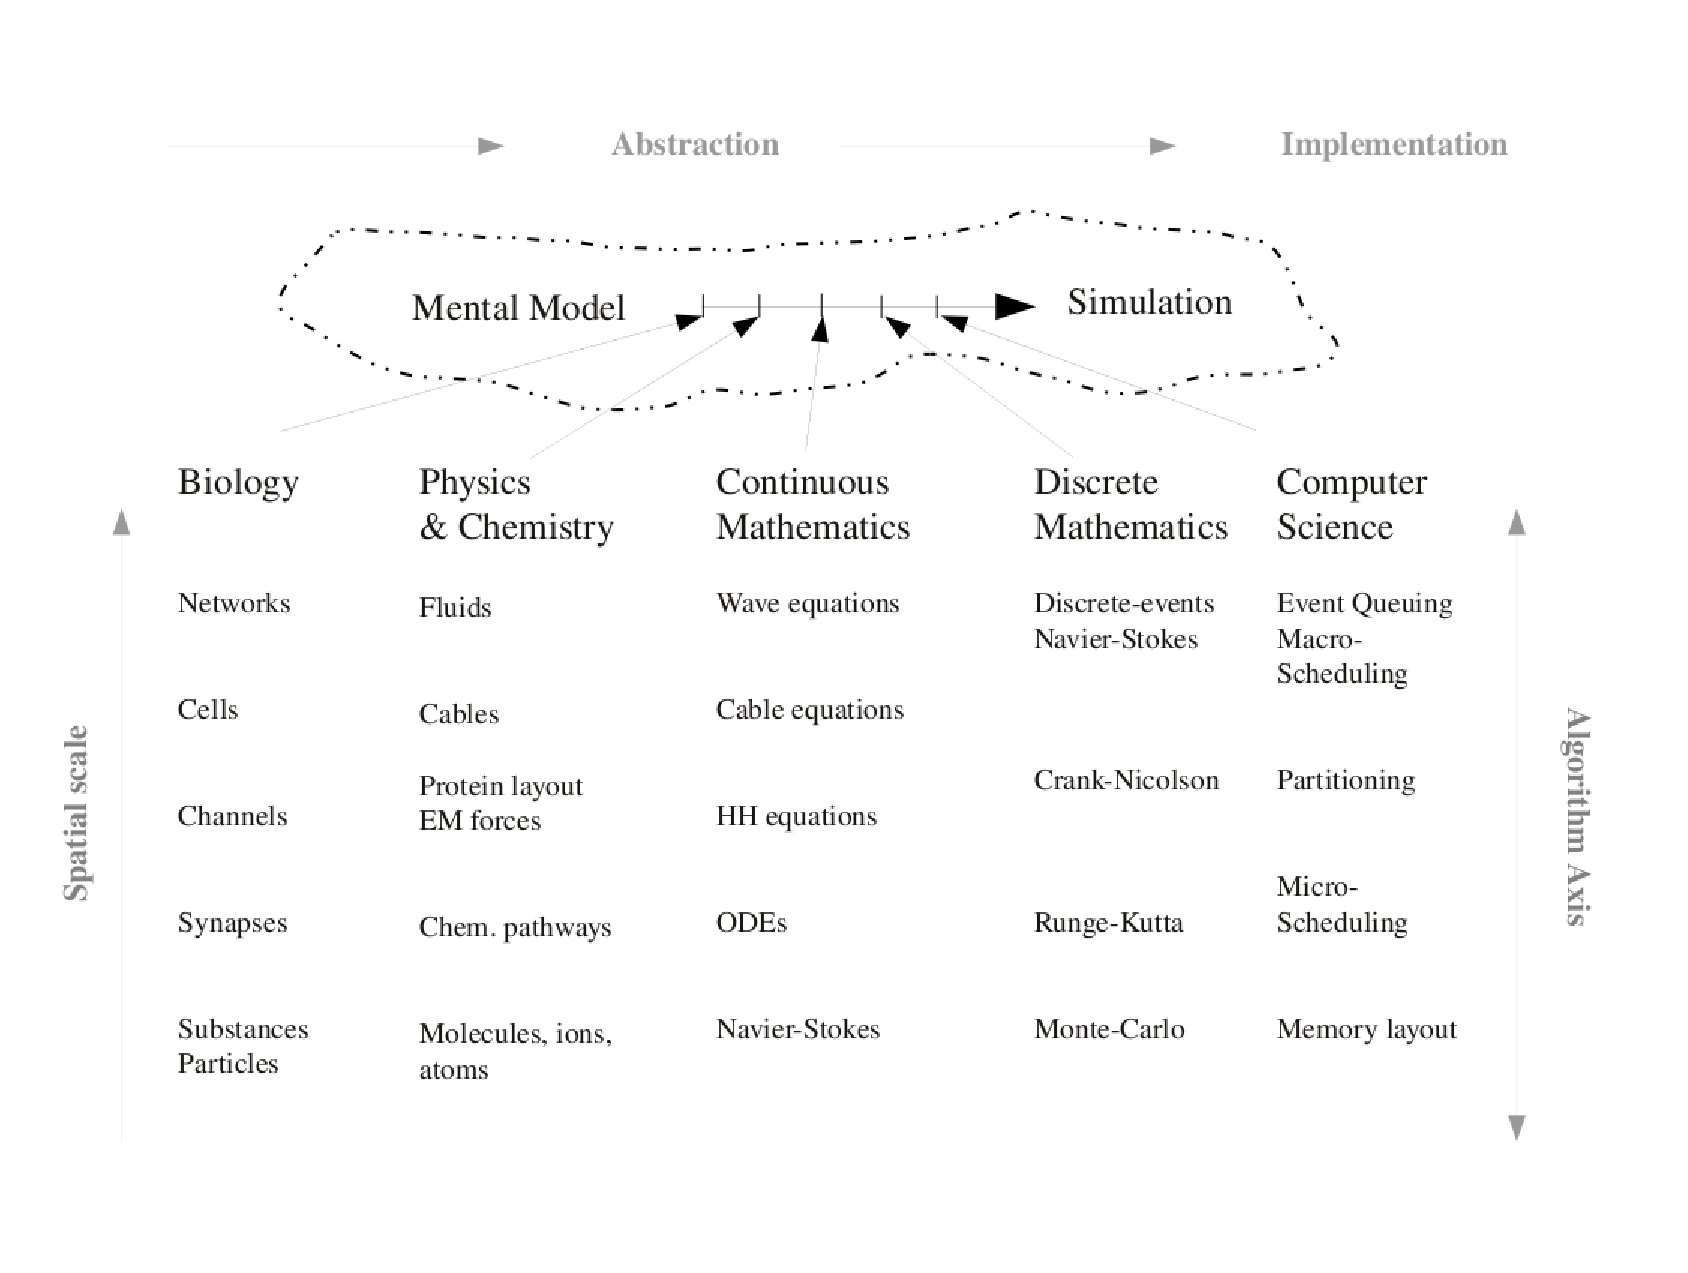
\includegraphics[width=0.75\textwidth]{figures/NS-abstraction-implementation.eps}
  \end{center}
  \caption{ \small{\bf Examples of different cognitive paths from mental model to simulation for different spatial scales.}  Each horizontal path first abstracts the model to a mathematical representation.  This is then followed by how this mathematical representation is implemented in computer software.  The different spatial scales at the left result in the requirement for different algorithms when implementing the computer software.  Each graphical representation of a research topic in the model taxonomy results in researchers applying several cognitive paths that are specific to their methodological workflows (as opposed to their mathematical solutions).  As a consequence the integration of (the results of) different research topics in the model taxonomy requires to trace back on the these cognitive paths.  }
  \label{fig5}
\end{figure}

The multidimensional framework implied by Figures~\ref{fig4} and~\ref{fig5} is based on the relationships between the schemas outlined by Marr, C\&S and the user and cognitive workflows described here. These relationships are used to develop a novel and simplifying approach to the simulation of scale-independent models. The results of application of the foregoing workflows and schemas in the identification and elaboration of a principled separation of concerns (see for example~\cite{Dijkstra:1982fu}) is explored further in the following section.

\section*{Results}

Based on the foregoing descriptions and discussions of the multi-dimensional complexity associated with modelling biological structures and functions as ‘simple’ as a single neuron, the features of the reconfigured GENESIS simulator (G-3 -- http://genesis-sim.org) relevant for scale-independent simulation are described.  Together with several scripting examples, it is shown how primary components of G-3 transparently support scale-independent simulation within the various biological resolutions of cells, channels and synapses (see Fig.~\ref{fig4}). In short, G-3 provides a scale-independent framework for computational neuroscience that resolves both the problems associated with the emergence of monolithic software and the problems associated with multiscale simulation.

\subsubsection*{Structural Overview of the CBI Architecture}

The Computational Biology Initiative Federated Software Architecture (CBI architecture) is defined as a modular paradigm that places stand-alone software components into a set of logical relationships \cite{cornelis12}.

In doing so, it defines a modular framework that provides the
necessary parts of a simulator. The architecture takes its name from the Computational Biology Initiative at the University of Texas at San Antonio, where development was first initiated.

\begin{figure}[ht]
\begin{center}
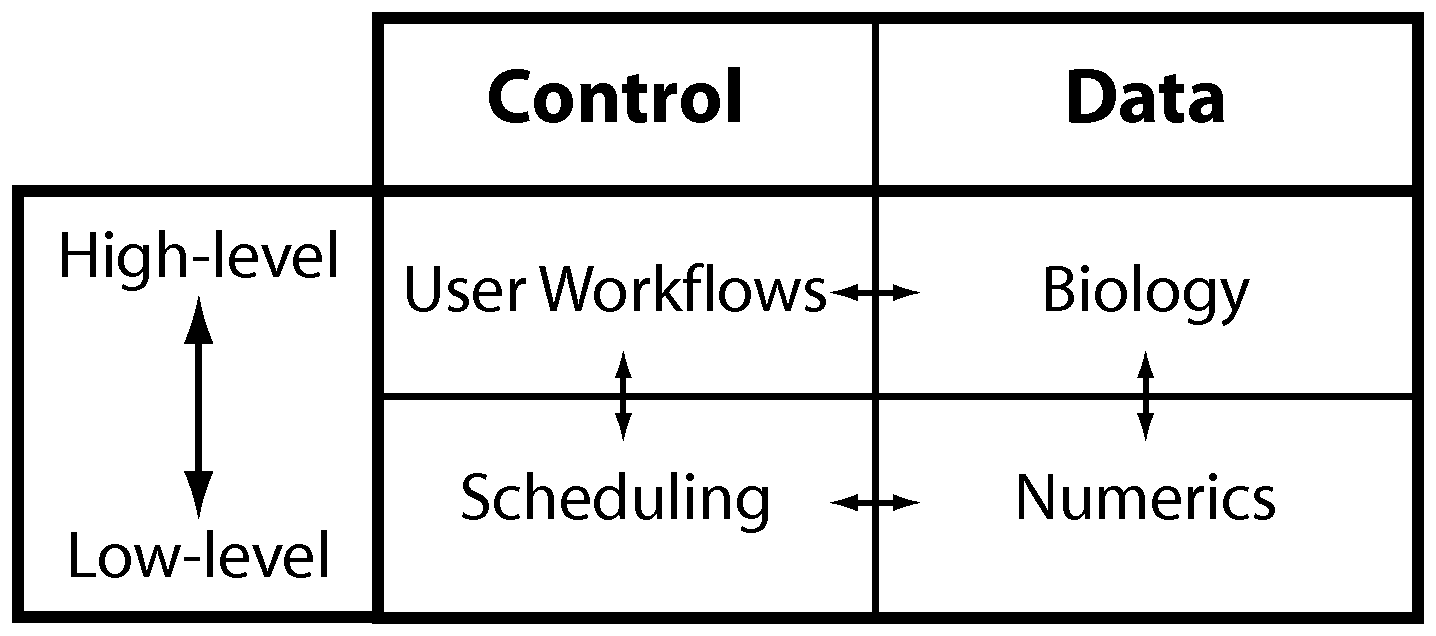
\includegraphics[width=0.75\textwidth]{figures/pone.0028956.g002.png}
\end{center}
\caption{\small{\textbf{Principle concerns.} The four fundamental building blocks of a simulator are distinguished by separating (i) Data from control and (ii) High level biological concepts from their mathematical implementation. In a federated architecture the only allowed interactions between modules are those indicated by the vertical and horizontal arrows. Diagonal interactions are forbidden as they ultimately lead to interactions that result in the evolution of a monolithic software architecture.}}
\label{fig6}
\end{figure}

A schema identified by separation of concerns (Fig.~\ref{fig6}, see \cite{cornelis12} for details) is expanded in Figure\,\ref{fig7} to give the modules that form the building blocks of the CBI architecture.  The schema retains the four quadrants of simulator functionality identified by the separation of concerns, including separation between control and data  and the notions of high-level representations for biology and low-level data for numerics (Fig.~\ref{fig7}: indicated by vertical and horizontal dashed lines, respectively).

Notably, the integrity of the simulator is maintained by only allowing interactions between vertically and horizontally located modules. Diagonal interactions are forbidden as they foster the mixing of functionality across different resolutions and typically lead to monolithic software applications. Ultimately, it is this partitioning of simulator functionality that lies at the core of simulator extensibility and provides the architectural foundation for transparent scale-independent simulation.

\begin{figure}[ht]
\begin{center}
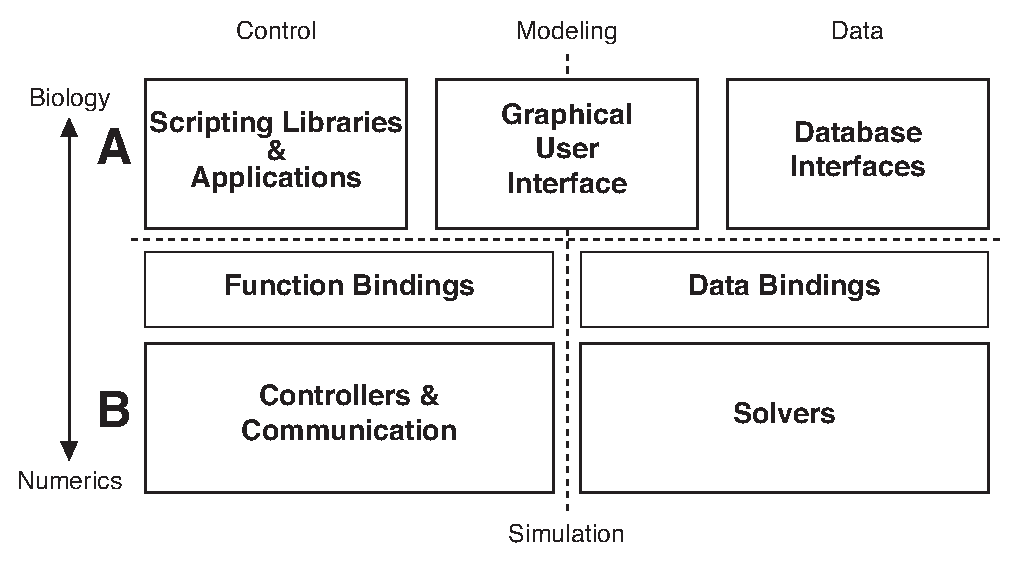
\includegraphics[width=0.75\textwidth]{figures/cbi-architecture-simple.eps}
\end{center}
\caption{ \small{\bf Overview of a Federated Software Architecture:}
  The primary functional modules defined for the CBI federated software architecture are illustrated.  Control modules are given to the left and data modules to the right.  A. The top layer contains conceptual data and controls representations of the biology of a model. B. The bottom layer contains representations that are
  numeric and thus close to the hardware.  The middle or intermediate layer bridges between these `biological' and `numerical' layers in a CBI compliant simulator. Importantly, Control (Scripting Libraries \& Applications) and Data (Database Interfaces) modules can interact either directly or via the Graphical User Interface. }
\label{fig7}
\end{figure}

The CBI architecture is referred to as being `federated' as it extends the modular approach associated with the development of single applications to the functional integration of otherwise independent applications. Federation aims to provide a unified interface to diverse applications and ideally make them look like a single
system to the user. In doing so, it provides transparency, heterogeneity, a high degree of function, autonomy for the underlying federated sources, extensibility, openness and the possibility of highly optimized performance (see \cite{federated-2002-xyz}). Here, extensibility is defined as a system design principle where an implementation takes into consideration future developments. An extensible system is one that includes mechanisms for expanding or enhancing the system with new capabilities without having to make major changes to system infrastructure. 

Enhanced application interoperability and performance is available through the use of flexible high-level scripting languages that support diverse workflows, low-level application programmer interfaces (API)s and application binary interfaces (ABI)s (see \cite{Cornelis:2011fk}).

% For completeness, we note that northbound and southbound interfaces
% are indicated in this figure. Northbound interfaces conceptualize
% lower level details, whereas, the southbound interfaces decompose
% the concepts in technical details, which are mostly specific to a
% single component of a software architecture. Northbound interfaces
% normally communicate with southbound interfaces of higher level
% components and vice versa. By convention, north- and southbound
% interfaces are drawn at the top and bottom of an architectural
% overview, respectively.

In summary, the CBI architecture provides a template for software development that, at its core, contains a simulator.  Additionally, the modularity and layering of the architecture simplifies connection to independent applications related to model construction and instantiation and the analysis and display of simulation output.

\subsubsection*{Behavioural View of the CBI Architecture}

Figure \ref{fig8} expands Figure \ref{fig7} to give more detail of the structural relationships between the different modules and sub-modules of the CBI architecture (previously described in \cite{cornelis12}). The behavior of the CBI architecture is defined by the functional and dynamic connectivity provided by these individual modules. This behavior is now introduced within the context of the user workflow.

\begin{figure}[h!t]
  \begin{center}
    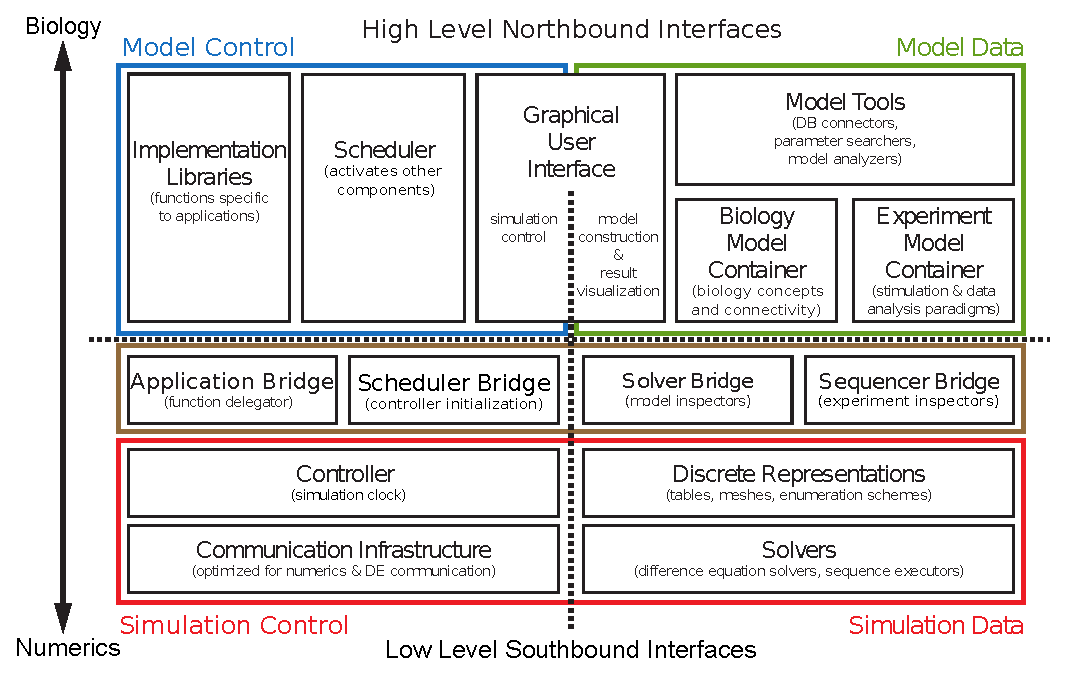
\includegraphics[width=0.75\textwidth]{figures/cbi-architecture-expanded.eps}
  \end{center}
  \caption{{\small{\bf Detailed view of the Computational Biology Initiative Federated Software Architecture} within each of the primary functional modules given in Figure \ref{fig7} are illustrated.  North bound interfaces group and conceptualize the details of the modules and interact with south bound interfaces of higher level modules.  Steps 1--3 of the user workflow induce data cycling between the upper layers (blue and green boxes) and lower layers (red box), see Fig.\,\ref{fig4} for details. Ultimately, the two layers interact to implement a single simulation. By design, any type of model including multiscale models will exhibit this data cycle. In contrast to previous versions of GENESIS and other neuronal simulation platforms, the design of G-3 is fundamentally modular, separating different functional components of the simulator into their own modules. Importantly, G-3 separates model descriptions from their mathematical representations.  This simplifies the implementation of new {\bf Solvers} and other run-time software components. The communication infrastructure connects different {\bf Solvers} to simulate different parts of a model and can `upscale' or `downscale' numerical data as needed. Additional detail is given in \cite{cornelis12}.}}
  \label{fig8}
\end{figure}

During the phase of model construction prior to simulation, users combine models from files and databases.  When the simulation runs, the numerical {\bf Solvers} perform the calculations of a simulation and save the output back to files and databases.  When these two steps are combined they imply a cyclic data flow from files and databases to the {\bf Solvers}.
%  Here we explain how user actions and data flows relate to one another in the CBI architecture and define the overall behavior of an implemented software system.

In more detail, as a result of Steps 1--3 of the user workflow (construct model, design experiment, run simulation, see Fig~\ref{fig4}), data flows both through and between software components. The cycle described here is for a single neuron simulation, however, all scales of model will exhibit similar activity.

Once Step 3 is completed, data generated by dynamic states of the model are available through databases and files. Consequently, there is no requirement to query software components that deal with numerical data. This provides an operational barrier to assist with preventing incremental conversion of a CBI compliant simulator to its monolithic equivalent.

In Step 4 of the user workflow (output), while maintaining the integrity of the separation of concerns, the availability of any model data from the {\bf Biology\,Model\,Container} and the functionality of {\bf Scripting\,Libraries\,\&\,Applications} can be used to connect the CBI architecture to external tools, for example Matlab (to implement output analysis).

At Step 5 of the user workflow (iterate), simulation output data and model parameters and structure available in the model containers can be combined, for example, to provide automated script generators for the creation of batch simulations. Importantly, at this stage of the workflow, the back-ends of the CBI architecture (indicated below the dotted horizontal line in Figures \ref{fig7} and \ref{fig8}) are unavailable. 

\subsection*{GENESIS 3.0}

The software architecture developed for G-3 supports a capacity for federated and modular software development that directly enables multiscale modelling.  Furthermore, its structure also supports the direct interaction with, or embedding of, models at different resolutions.  During model construction this is accomplished through the reconfiguration of the internal model storage format, while during simulation run-time it occurs through specific software modules that create intermediary representations of variables present at multiple resolutions (described in more detail below).

Several explicit features of G-3 allow new software components to be rapidly incorporated into the simulator: (1) modularity of the CBI architecture supports the development of new {\bf Solvers} independently of other software components. This encourages full focus on the mathematical aspects of {\bf Solvers} and their implementation and leads to better optimization, (2) the {\it Developer\,Package} facilitates integration of new {\bf Solvers} into the build system of G-3 enabling immediate regression testing, (3) easy extension of the configuration of the internal model storage format to establish new declarative model tokens and parameters recognized by new {\bf Solvers}, (4) easy construction of an interface between the internal data storage format and the core of new {\bf Solvers} and finally, (5) a communication software component that creates simulation run-time interfaces between {\bf Solvers}.

Solvers currently available in G-3, starting at the highest level, include: {\bf DES}, a discrete event queuing and distribution infrastructure for network modelling, {\bf Heccer}, a single neuron solver, {\bf Chemesis-3}, a simple reaction-diffusion system solver and {\bf Experiment}, which provides simulation-time components for current injections, time-tables and output.

\subsection*{Scale-Independent Scripting}

In  a typical multiscale model different numerical solution methods are required to solve the different types of mathematical equations associated with the different scales of the model.  In G-3 the cable equation and ion currents are numerically solved with implicit Crank-Nicolson integration using {\bf Heccer}.  Calcium models are numerically solved with {\bf Chemesis-3}. The association between a given model and its {\bf Solvers} can be configured by the user.
%Under planned extensions to the G-shell syntax, the correct syntax
%for a loaded single neuron model with name "/Purkinje" would be:
%For example to associate the model named ``/Purkinje'' with the solver {\bf heccer}, the command is:

%\begin{tiny}
%\begin{verbatim}
%  solverset "/Purkinje => heccer"
%\end{verbatim}
%\end{tiny}

%To use {\bf Chemesis-3} to simulate a complex network model of biochemical %pathways, here called {\it cal1}, a user would type in the G-3 shell:

%\begin{tiny}
%\begin{verbatim}
%  solverset "/cal1 => chemesis3"
%\end{verbatim}
%\end{tiny}

In the case where a network of biochemical pathways is defined inside a single neuron model, a user would employ two commands with wildcards to associate the correct solver with each component of the model.%%, for example:

%\begin{tiny}
%\begin{verbatim}
 % solverset "/**/cal1 => chemesis3"
%  solverset "/Purkinje/**[!cal1] => heccer"
%\end{verbatim}
%\end{tiny}

% For figure citations, please use "Fig" instead of "Figure".
%Nulla mi mi, Fig~\ref{fig1} venenatis sed ipsum varius, volutpat euismod diam. Proin rutrum vel massa non gravida. Quisque tempor sem et dignissim rutrum. Lorem ipsum dolor sit amet, consectetur adipiscing elit. Morbi at justo vitae nulla elementum commodo eu id massa. In vitae diam ac augue semper tincidunt eu ut eros. Fusce fringilla erat porttitor lectus cursus, \nameref{S1_Video} vel sagittis arcu lobortis. Aliquam in enim semper, aliquam massa id, cursus neque. Praesent faucibus semper libero.

% Place figure captions after the first paragraph in which they are cited.
%\begin{figure}[!h]
%\caption{{\bf Bold the figure title.}
%Figure caption text here, please use this space for the figure panel descriptions instead of using subfigure %commands. A: Lorem ipsum dolor sit amet. B: Consectetur adipiscing elit.}
%\label{fig1}
%\end{figure}

% Results and Discussion can be combined.
%\section*{Results}
%Nulla mi mi, venenatis sed ipsum varius, Table~\ref{table1} volutpat euismod diam. Proin rutrum vel massa non gravida. Quisque tempor sem et dignissim rutrum. Lorem ipsum dolor sit amet, consectetur adipiscing elit. Morbi at justo vitae nulla elementum commodo eu id massa. In vitae diam ac augue semper tincidunt eu ut eros. Fusce fringilla erat porttitor lectus cursus, vel sagittis arcu lobortis. Aliquam in enim semper, aliquam massa id, cursus neque. Praesent faucibus semper libero.

% Place tables after the first paragraph in which they are cited.
%\begin{table}[!ht]
%\begin{adjustwidth}{-2.25in}{0in} % Comment out/remove adjustwidth environment %if table fits in text column.
%\centering
%\caption{
%{\bf Table caption Nulla mi mi, venenatis sed ipsum varius, volutpat euismod diam.}}
%\begin{tabular}{|l+l|l|l|l|l|l|l|}
%\hline
%\multicolumn{4}{|l|}{\bf Heading1} & \multicolumn{4}{|l|}{\bf Heading2}\\ %\thickhline
%$cell1 row1$ & cell2 row 1 & cell3 row 1 & cell4 row 1 & cell5 row 1 & cell6 row 1 & cell7 row 1 & cell8 row 1\\ \hline
%$cell1 row2$ & cell2 row 2 & cell3 row 2 & cell4 row 2 & cell5 row 2 & cell6 row 2 & cell7 row 2 & cell8 row 2\\ \hline
%$cell1 row3$ & cell2 row 3 & cell3 row 3 & cell4 row 3 & cell5 row 3 & cell6 row 3 & cell7 row 3 & cell8 row 3\\ \hline
%\end{tabular}
%\begin{flushleft} Table notes Phasellus venenatis, tortor nec vestibulum %mattis, massa tortor interdum felis, nec pellentesque metus tortor nec nisl. Ut %ornare mauris tellus, vel dapibus arcu suscipit sed.
%\end{flushleft}
%\label{table1}
%\end{adjustwidth}
%\end{table}


%PLOS does not support heading levels beyond the 3rd (no 4th level headings).
%\subsection*{\lorem\ and \ipsum\ nunc blandit a tortor}
%\subsubsection*{3rd level heading} 
%Maecenas convallis mauris sit amet sem ultrices gravida. Etiam eget sapien %nibh. Sed ac ipsum eget enim egestas ullamcorper nec euismod ligula. Curabitur %fringilla pulvinar lectus consectetur pellentesque. Quisque augue sem, %tincidunt sit amet feugiat eget, ullamcorper sed velit. Sed non aliquet felis. %Lorem ipsum dolor sit amet, consectetur adipiscing elit. Mauris commodo justo %ac dui pretium imperdiet. Sed suscipit iaculis mi at feugiat. 

%\begin{enumerate}
%	\item{react}
%	\item{diffuse free particles}
%	\item{increment time by dt and go to 1}
%\end{enumerate}

%\subsection*{Sed ac quam id nisi malesuada congue}

%Nulla mi mi, venenatis sed ipsum varius, volutpat euismod diam. Proin rutrum %vel massa non gravida. Quisque tempor sem et dignissim rutrum. Lorem ipsum %dolor sit amet, consectetur adipiscing elit. Morbi at justo vitae nulla %elementum commodo eu id massa. In vitae diam ac augue semper tincidunt eu ut %eros. Fusce fringilla erat porttitor lectus cursus, vel sagittis arcu lobortis. %Aliquam in enim semper, aliquam massa id, cursus neque. Praesent faucibus %semper libero.

%\begin{itemize}
%	\item First bulleted item.
%	\item Second bulleted item.
%	\item Third bulleted item.
%\end{itemize}

\section*{Discussion}

% This Discussion section reflects the cognitive process of the authors active in the project described above.
Several features of the scientific exploration of reality have been raised in foregoing sections. Their  theoretical underpinnings are now further clarified to better delineate the implications for a better understanding of the structure and function of the mammalian central nervous system. To this end, it is useful to recall the plausible origins of a current widely accepted understanding of neural structure. This leads to what the authors propose will provide a better match between the known structures and functions of the mammalian central nervous system and the models employed to achieve greater understanding. Here, it is useful to paraphrase what Dijkstra~\cite{Dijkstra:1982fu} wrote over forty years ago: Essentially, this discussion contains nothing new; on the contrary, its subject matter is so old that sometimes it seems forgotten. It is written in an effort to undo some of the more common misunderstandings that are encountered on a nearly daily basis in the professional world of theoretical neuroscience. As will be shown here, the adjective ``scientific" when used in the expression ``scientific thought" refers more to a {\it{way}} of thinking than to {\it{what}} the thoughts are about. Many practitioners must feel that, in the case of theoretical neuroscience, scientific thought is a luxury that can be afforded in more established disciplines, but not in the intellectual wilderness they now found themselves in. However, scientific thought is not a luxury made possible in established scientific disciplines, on the contrary: it is the tool that makes the establishment of those disciplines possible.

Dijkstra further notes what he considers to be a characteristic feature of intelligent thinking: It is the willingness to study in depth an aspect of the given subject matter in isolation for the sake of its own consistency, all the time knowing that one is occupied only with a single aspect as, in computer science and particularly software development, history shows that nothing is gained by tackling various aspects of a problem simultaneously. It is the sole purpose of the specifications identified by a principled ``separation of concerns" to act as the interface between a system's developers and users. The task of ``making a thing satisfying our needs" as a single responsibility has two parts: ``stating the properties of a thing, by virtue of which it would satisfy the required needs" and ``making a thing guaranteed to have the stated properties." In short, the current state of theoretical neuroscience is a mess that has been caused by too much unscientific thought.

As recent publications report, current models in theoretical neuroscience reveal a fundamental contradiction in the proposal to adopt a pragmatic perspective (see for example~\cite{levenstein23}). Implicitly, this leads to the employment of an utilitarian approach: Like their mechanistic counterparts, normative explanations establish links between descriptions; descriptions which each have their own utility for different problems by virtue of their unique abstractions. It is the involvement of utilitarianism that injects one of the most powerful and persuasive approaches to normative ethics in the history of philosophy~\cite{driver22}, that of consequentialism; itself the paradigmatic case of utilitarianism~\cite{sinnott-armstrong22}. As classic utilitarianism reduces all morally relevant factors to consequences, it is actually a complex combination of many distinct claims~\cite{sinnott-armstrong22}. Thus, consequentialism is both historically important and still a popular theory which embodies the basic intuition that what is best or right is whatever makes the world best in the future, as the past cannot be changed~\cite{sinnott-armstrong22}. In short, these philosophical conclusions introduce a strong case for a moral underpinning to science.

Such an approach is further predicated on the notions of a {\it{Celestial Hierarchy}} that took over 1,000 years to evolve into the idea of  the {\it{Great Chain of Being}}.

\subsection*{The Problems with Simulators}

At the core of the problem is the lack of distinction in many contemporary simulators made between biological data, numerical data and control operations during the software architecture development stage of simulator design. The majority of such simulators remain primarily focused on the biological and mathematical aspects of a model. As they do not respect all three of Marr's levels, i.e. the third of Marr's levels (``hardware'' implementation) is not addressed during software design, the complexity of multiscale simulation is greatly increased.

Just as the `hardware' of a biological system should be accounted for in the cognitive process of model development, so must it be accounted for during the simulation of the model. In a simulator this can be achieved by the software architecture and its organization of simulator functionality. Making the cognitive model concordant with simulator functionality removes many of the problematic aspects of multiscale modeling.

This is particularly the case as theoretical models do not exist in a vacuum. They are part of larger social, cultural and anthropological structures. As such and as noted here, at a deeper level, theoretical models are embedded in the evolutionary process as it is expressed in human neural and mental activity~\cite{jacobson93}.

\subsection*{The Multiscale Problem}

While seeming both transparent and widely accepted, some authors consider a careful definition of the term multiscale should be identified as it is a recent notion that very quickly spirals into a realm of catch-all scientific jargon (for example~\cite{walpole13}). That such freedom is encouraged is evidenced by the absence of the term from \textit{The Encyclopedia of Computational Neuroscience}~\cite{jung22}, where nine years after its initial publication there is neither section nor article devoted to the difficulties of multiscale computation. More trivially, the term appears on ten occasions in the 3,663 pages of the second edition and also in a total of twelve publication titles cited in the References that follow each entry in the Encyclopedia.

Historically, multiscale modelling has primarily been explored in the fields of engineering, computer sciences and physics, where multiple scales of observation have motivated extensive use of this approach. More recently, computational neuroscience has shown an increased interest in this discipline. It is now recognised as being essential for a better understanding of nervous systems and how molecular level neuronal events modify underlying neural circuits and brain function, thus both innate and learned behaviours~\cite{bouteiller11}.

Founded on the widely accepted paradigm exemplified in Figure\,\ref{fig1} that the central nervous system is a highly hierarchical structure that integrates several spatial and temporal levels of complexity~\cite{bouteiller11}, the concept of multiscale modelling has been implemented by employing different models, possibly described by different physical formalisms and acting simultaneously on different temporal and spatial scales, so as to study important features of complex phenomena at multiple levels of organization~\cite{djurfeldt07}.

Thus, a multiscale model typically accounts for more than one magnitude of resolution across discriminable functional domains~\cite{walpole13}. However, many models of physical systems implicitly account for multiple resolutions by simplifying their boundary conditions\marginpar{\scriptsize Needs one sentence more explanation?} into “black boxes” where assumptions about other spatial or temporal domains are summarized by governing equations. Further, explicitly modeled tiers of resolution must also provide additional information unobtainable by independent exploration at a single resolution. This latter requirement is one that enables a fundamentally important distinction to be made between explanatory models and mere demonstrations. Notably, in a similar way, respectively, a theory provides an explanation, whereas, a law provides a description~\cite{schurger22}.

\subsubsection*{Historical and Cultural Foundational Factors}

The problems elaborated around Fig~\ref{fig1} can be attributed to the confluence of several foundational factors. These include the cumulative effect of historical assumptions that have evolved from Platonic, Aristotelian and Neo-Platonic~\cite{parker99} philosophy. They have undergone refinement during the Neo-Platonic and Medieval Periods such that, by the time of the Elizabethan Period~\cite{tillyard17} and the subsequent Enlightenment, they develop into increasingly profound and culturally entrenched metaphysics that constitute essential presuppositions in the framing of scientific hypotheses~\cite{lovejoy48}.

=== rewrite 1, for the discussion

Historically, the idea of hierarchy to organize scientific processes and knowledge may have been introduced in the late Medieval periods when the Great Chain of Being was used to order and describe all matter and life and introduced the levels, attributes and hence roles of life.  It spanned a possibly infinite range of levels from inert matter to humanity and beyond through realms of angels, to ultimately reach God. Thus, this hierarchical framework provided an unquestionable organizational paradigm for developing a science based understanding of the world.  It provided the underpinnings of science during its rapid expansion in the period of the Enlightenment.

The idea of the Great Chain of Being was heavily intertwined with the more theological idea of the Celestial Hierarchy that defined humanity's relation to God that predates the former idea.

=== original, for the discussion

This process structured foundational theological beliefs~\cite{lovejoy48} that then became subsumed by the rapid expansion of science during the Enlightenment to become foundational beliefs driving cognitive understanding and organization of the developing biological sciences. Subsequently, these theological beliefs and metaphysical assumptions came to form some of the most powerful dogmas of the neurosciences and particularly the theoretical and mathematical implementations that underwrote the computational and simulation neurosciences. In short, a theological Celestial Hierarchy~\cite{parker99} that defined humanity's relation to God was subsumed into a Great Chain of Being that ordered and described the levels, attributes and hence roles of life, in a hierarchy that spanned a possibly infinite range of levels from inert matter to humanity and beyond through realms of angels, to ultimately reach God. Thus, a hierarchical framework originating in a theological world view has come to provide a central dogma acting as an organizational paradigm for understanding the structure of the human central nervous system.

=== end original

In what might be referred to as some of the central assumptions of the classical approach to the study of neuroscience, understanding how any system works requires four things~\cite{swanson15}: (1) A general understanding of what the system does, (2) a parts list, (3)an account of how each part works and (4) knowledge of how the parts are interconnected to function as a whole. That such issues are assumed foundational was earlier reinforced by statements such as: The nervous system is a biological computer integrating the body’s reflex and voluntary environmental interactions (behavior) with a relatively constant internal state (homeostasis)--promoting survival of the individual and species~\cite{swanson10}.

Such a classical perspective only continues to be further reinforced by (for example) theoretical propositions such as the ``power-of-two'' postulate~\cite{tsien15}. This describes a specific-to-general combinatorial connectivity logic, that provides a radically different wiring logic organizing the microarchitecture of cell assemblies. It is hypothesised to give a basic computational principle that readily enables knowledge and adaptive behavior to emerge from a genetically programmed, preconfigured wiring logic that inherently enables knowledge and adaptive behaviors to emerge much more readily upon learning.

% Similarly, an analysis of the primate visual system has reported 32 neocortical and associated visual areas and 305 sets of connectivity amongst them. It also included 14 levels of visual processing, if extra-cortical areas such as the retina, lateral geniculate nucleus, entorhinal cortex and hippocampus were included~(see Fig.\,4~\cite{felleman91}). 

% The sheer number of known cortical connections raises the specter of a network so complex and chaotic as to be virtually impossible to decipher~\cite{vanessen93}. Although, some order has been introduced by the fact that anatomically, nearly all of the appropriately examined pathways can be arranged as reciprocal pairs. Further, the great majority of such connectivity show a striking asymmetry in laminar organization. However, as proposed by~\cite{mcculloch45a,mcculloch45b}, such circuits are better understood not as a symptom of hierarchical, but rather a feature of heterarchical functional organization.

% GENESIS was one of the first general purpose open source software platforms designed to support the simulation of neural systems ranging from subcellular components to system-level models (see http://genesis-sim.org). It first became available in 1988, with a full public release in 1990, followed in 1995 by GENESIS version 2.0~\cite{jung22}. In 2014 the final packaged version of GENESIS (version 2.4) was released with any further community development made available from the Repository for Continued Development of the GENESIS 2.4 Neural Simulator (https://github.com/genesis-sim/genesis-2.4). Almost thirty-five years after its public release an augmented GENESIS 2.4 continues to provide a world-leading open source realistic neural simulation platform~(see Table\,1 in \cite{tikidji-hamburyan17}).

% The innovative beginnings of GENESIS were based on a number of assumptions with regard to the aims of computational neuroscience. These assumptions included, amongst others: (1) The construction of ``realistic" computer models based on actual anatomy and physiology is an essential prerequisite for understanding the computational organization of the nervous system, (2) Understanding nervous system function depends upon being able to construct and link models at many different levels of biological scale, (3) Growth of a modeling system is reliant on the ability of individual modelers to develop and share model features and components, (4) The system should be as machine independent as possible and (5) Successful use depends on a graphical interface that supports users with different ranges of computer expertise.

% More than a decade prior to the release of GENESIS 2.4, it was realized that rather than just component modularity, what was required for a simulation package in computational neuroscience was a collaborative system~\cite{cornelis03}. In such a system a small extensible core or kernel manages a set of modules and components that engage in shared activities via semantically defined interfaces. In the absence of such a software architecture even the most valiant coding efforts in computational neuroscience were found to ultimately result in what might be referred to as a monolithic software architecture. In such an architecture it is difficult to extend a simulation platform and it becomes increasingly difficult to construct and simulate complex neuronal models even when their size and complexity is only incrementally increased.

% It was found that a major reason forcing the evolution of a software platform into a monolithic architecture occurs when the data model employed is insufficient to account for all the requirements of a realistic model. Typically, this occurs when the mathematical implementation of a model looses its conceptual dimension. This puts pressure on the cognitive model developed by an investigator. It results from the fact that they are forced to think about the computational model in a mathematical way as it is actually instantiated by code that not only constructs all required neural populations but also the links necessary for the network connectivity of individual neurons.

% In more detail, the problems of a monolithic software architecture emerge as the hierarchical function and three-dimensional nature of a complex cognitive model is incorporated into ever-larger computational simulations. Following the model setup phase, both the topology of the network and the projections between the various populations typically are lost. This occurs when the projections and connections of individual neurons exist within and between different levels of the network hierarchy, yet all connections require inspection at each stimulation timestep. Ultimately, this is a problem that is only exacerbated as neuronal populations are enlarged, whereby each constituent neuron becomes both source and target for increasing connectivity.

\subsection*{The Celestial Hierarchy and The Great Chain of Being}

It has been proposed here that the multiscale problem, at its origin, started with the idea of {\it The Great Chain of Being}. {\it The Great Chain of Being} is a hierarchical structure of all matter and life, thought by medieval Christianity to have been decreed by God. It begins with God and descends through angels, humans, animals and plants to minerals. The idea extended across more than two millennia and together with its axiomatic principles of, ``plenitude,' ``continuity'' and ``graduation," from the time of Plato was one of the most famous in the vocabulary of Western theology, philosophy and science~\cite{lovejoy48}. Until about the 1850s, it was probably the most widely familiar conception of the general scheme of things and of the constitutive patterns of the universe. As such, it has necessarily come to predetermine current ideas on many other matters both social and scientific.  One hundred years later, in the middle of the twentieth century, it was recognised as a concept that had become one of the half-dozen most potent and persistent presuppositions in Western thought.

The idea of a hierarchical chain of levels can be seen as an example par excellence of a simplifying organizational principle whereby to understand cerebral cytoarchitecture, i.e. the cognitive model, but also provides an organizational framework that enables understanding thus principled model implementation based on hierarchical frameworks encapsulating levels of organization and function associated with the neural structures observed within the anatomy of the mammalian central nervous system. The approach seems to continue to predetermine and drive much ongoing theory and many ideas considered fundamental concerning the understanding of nervous system function.

%Nulla mi mi, venenatis sed ipsum varius, Table~\ref{table1} volutpat euismod %diam. Proin rutrum vel massa non gravida. Quisque tempor sem et dignissim %rutrum. Lorem ipsum dolor sit amet, consectetur adipiscing elit. Morbi at justo %vitae nulla elementum commodo eu id massa. In vitae diam ac augue semper %tincidunt eu ut eros. Fusce fringilla erat porttitor lectus cursus, vel %sagittis arcu lobortis. Aliquam in enim semper, aliquam massa id, cursus neque. %Praesent faucibus semper libero~\cite{bib3}.

\subsection*{Theories in Neuroscience as Emergent Property of Cognitive Models}
From such a perspective, it is quite remarkable that in the earliest phase of the Common Era of the third millennium (the twenty-first century), the foundations of biological science and in particular theories in neuroscience still appears to be an emergent property of a cognitive model introduced by Plato and subsequently elaborated into a theological world view as the {\it{Celestial Hieriarchy}}, otherwise known as the {\it{The Great Chain or Being}}. In its current evolution it seems to have been forgotten that, (1) theories in neuroscience are mental models fabricated to explain the meanings of observations of nervous systems and (2) that neuroscience is founded on the assumption that our models are more or less true representations of some objective reality~\cite{jacobson93}.

\subsection*{C\&S's Position}

Whether unintentional or not, C\&S's position appears to provide a secular interpretation of the theology of {\it{The Celestial Hierarchy}} and its more scientific interpretation, {\it{The Great Chain of Being}}. The framework developed by C\&S, can be seen as an example {\it{par\,excellence}} of a simplification of cerebral cytoarchitecture that acts to reinforce a long-standing metaphysical organizational framework. A framework that continues to provide the predominant understanding of the principles of neural structure and function in the mammalian central nervous system. It is one that appears to remain firmly embedded in a metaphysical framework that provides a core principle of classical organizational dogma in the biological sciences. It espouses hierarchical levels of organization and function and is a paradigm that necessarily continues to predetermine much ongoing theory and many ideas considered fundamental to increased understanding of biological systems in general and those that contain nervous systems in particular.


\subsection*{Past Impediments to Scientific Progress}

It has been stated that: Science as an institutionalized art of inquiry has yielded varied fruit with its currently best-publicized products undoubtedly the technological skills that have been transforming traditional forms of human economy at an accelerating rate~\cite{nagel61}.

It is, however, timely to remember that such a sanguine view of the change wrought by scientific inquiry seems to ignore the existence of still-ongoing  institutional and cultural impediments. Impediments that began with some of the earliest metaphysical and scientific investigations and that have continued to be erected into the modern era. Some of these are now given.

Initially in the physical sciences and astronomy in particular, Copernicus' {\it{On the Revolutions of the Heavenly Spheres}} (1543), was banned on religious grounds. Galileo was prosecuted by the Inquisition in 1633 and condemned to house arrest until his death for publication of {\it{Dialogue Concerning The Two Chief World Systems}} (1632); a process likely set in motion almost a quarter of a century earlier by his publication of {\it{Starry Messenger}} (1610).

It therefore comes as little surprise that just over 120 years later in 1755 Kant~\cite{kant08} was motivated to open the preface to his {\it{Universal Natural History And Theory Of The Heavens}} (republished~\cite{kant08}) by warning that he has: Chosen a subject which is capable of exciting an unfavourable prejudice in a great number of readers at the very outset, both on account of its own intrinsic difficulty and also from the way it may be regarded from the point of view of religion.
 
In a similar vein, just over a further 100 years later, in an Encyclopedia Britannica entry concerning Vaccination, Creighton wrote that~\cite{creighton88}: It is right to say that the views expressed in the present article diverge in many points from the opinions generally received among medical men and must be regarded not as the exposition of established and undisputed doctrine, but as the outcome of an independent and laborious research.

More recently, with regard to the scientific process itself, negative sentiments were initially aroused by the publication of Kuhn's {\it The Structure of Scientific Revolutions} (first published 1962, see~\cite{bird22}).

Although the foregoing examples may appear isolated and idiosyncratic in their time, this is not necessarily the case. Two significant contemporary examples, specific to  computational neuroscience in particular, are now given. The first occurred when scientific advance appeared to be consciously impeded by universities. This was avoided by clever naming by computer companies which allowed investigators to circumvent unsuspecting university purchasing offices, agents of computing committees, who wanted to keep control over campus computing mainframes~\cite{Moore:2010vn}. Campus researchers could easily order a PDP because this name was not recognized as being a computer. Consequently, investigators were able to “stealth purchase” computers during the 1960s and were helped by computer manufacturers to bypass university computer committees who were road-blocking access to research tools.

The second example is provided by a recent report, issued following the introduction of the Human Brain Project in Europe~\cite{mahfoud21} It showed that competing visions of how brain models should be built became tied to debates over how scientific communities should be governed. Discussion concerned whether models and the scientific communities that create them, should be unified rather than pluralistic. Ultimately and possibly rather unsurprisingly echoing Sperry~\cite{sperry80}, it was concluded that scientific models are a focus of contention that mirror socio-political tensions associated with imagined social and political futures of either unification or pluralism.


\subsection*{Releasing the Historical Constraints}

In contradistinction to the core beliefs, proposals and observations extant within the biological sciences, along with their now problematic nature, an alternative is posited here that has resolved significant aspects of the problems of multiscale modelling and monolithic software code currently faced by computational and simulation neuroscience. Based on notions of heterarchy, the reconfiguration of the GENESIS simulator has provided a foundation for an alternative world view where ordered hierarchical assumptions and the teleology of cause and effect are replaced by the heterarchical relational interactions of change and consequence. In turn, this leads to explanations of phenomena not in terms of the purpose they serve (the hierarchical assumption), but rather in terms of how they arise (the heterarchical proposition).

It is further postulated that such a pivot in viewpoint releases neuroscience from the historical constraints of an outdated worldview. A once sufficient worldview based on a now maladaptive perception that assumed hierarchical organization provided the organizational structure of functionality and mechanism that lay dormant awaiting discovery in the biological sciences.

Along with the foregoing point, some of the historical issues that have arisen with the development of realistic models employed for the computational simulation of neurophysiology have briefly been introduced. In the process, dominant classical conceptual paradigms of computational and simulation neuroscience have been revisited.

Given the examples of theo-philosophical and socio-political impediment briefly mentioned in this Introduction; in concluding, it is perhaps timely to remember that less than 50 years ago Sperry wrote~\cite{sperry80}: In attempting to understand brain physiology and function, at stake are central key concepts that directly involve fundamental convictions regarding the nature of man's inner being, physical reality, the meaning of existence and related matters of ultimate concern. Further, that perspectives in this area profoundly shape human value systems and societal decision-making and hence human destiny.

\section*{Conclusion}

%CO\textsubscript{2} Maecenas convallis mauris sit amet sem ultrices gravida. %Etiam eget sapien nibh. Sed ac ipsum eget enim egestas ullamcorper nec euismod %ligula. Curabitur fringilla pulvinar lectus consectetur pellentesque. Quisque %augue sem, tincidunt sit amet feugiat eget, ullamcorper sed velit. 

%Sed non aliquet felis. Lorem ipsum dolor sit amet, consectetur adipiscing elit. %Mauris commodo justo ac dui pretium imperdiet. Sed suscipit iaculis mi at %feugiat. Ut neque ipsum, luctus id lacus ut, laoreet scelerisque urna. %Phasellus venenatis, tortor nec vestibulum mattis, massa tortor interdum felis, %nec pellentesque metus tortor nec nisl. Ut ornare mauris tellus, vel dapibus %arcu suscipit sed. Nam condimentum sem eget mollis euismod. Nullam dui urna, %gravida venenatis dui et, tincidunt sodales ex. Nunc est dui, sodales sed %mauris nec, auctor sagittis leo. Aliquam tincidunt, ex in facilisis elementum, %libero lectus luctus est, non vulputate nisl augue at dolor. For more %information, see \nameref{S1_Appendix}.

%\section*{Supporting information}

% Include only the SI item label in the paragraph heading. Use the %\nameref{label} command to cite SI items in the text.
%\paragraph*{S1 Fig.}
%\label{S1_Fig}
%{\bf Bold the title sentence.} Add descriptive text after the title of the item (optional).

%\paragraph*{S2 Fig.}
%\label{S2_Fig}
%{\bf Lorem ipsum.} Maecenas convallis mauris sit amet sem ultrices gravida. %Etiam eget sapien nibh. Sed ac ipsum eget enim egestas ullamcorper nec euismod %ligula. Curabitur fringilla pulvinar lectus consectetur pellentesque.

%\paragraph*{S1 File.}
%\label{S1_File}
%{\bf Lorem ipsum.}  Maecenas convallis mauris sit amet sem ultrices gravida. %Etiam eget sapien nibh. Sed ac ipsum eget enim egestas ullamcorper nec euismod %ligula. Curabitur fringilla pulvinar lectus consectetur pellentesque.

%\paragraph*{S1 Video.}
%\label{S1_Video}
%{\bf Lorem ipsum.}  Maecenas convallis mauris sit amet sem ultrices gravida. %Etiam eget sapien nibh. Sed ac ipsum eget enim egestas ullamcorper nec euismod %ligula. Curabitur fringilla pulvinar lectus consectetur pellentesque.

%\paragraph*{S1 Appendix.}
%\label{S1_Appendix}
%{\bf Lorem ipsum.} Maecenas convallis mauris sit amet sem ultrices gravida. %Etiam eget sapien nibh. Sed ac ipsum eget enim egestas ullamcorper nec euismod %ligula. Curabitur fringilla pulvinar lectus consectetur pellentesque.

%\paragraph*{S1 Table.}
%\label{S1_Table}
%{\bf Lorem ipsum.} Maecenas convallis mauris sit amet sem ultrices gravida. %Etiam eget sapien nibh. Sed ac ipsum eget enim egestas ullamcorper nec euismod %ligula. Curabitur fringilla pulvinar lectus consectetur pellentesque.

\section*{Acknowledgments}

Allan D. Coop commends the Australian and United States Federal Governments for their support of employable people through a Universal Basic Income.

\nolinenumbers

% Either type in your references using
% \begin{thebibliography}{}
% \bibitem{}
% Text
% \end{thebibliography}
%
% or
%
% Compile your BiBTeX database using our plos2015.bst
% style file and paste the contents of your .bbl file
% here. See http://journals.plos.org/plosone/s/latex for 
% step-by-step instructions.
% 

\bibliography{../tex/bib/2023-10-06-g3-refs-adc}
% \bibliography{bib/g3-refs-adc}

%%\begin{thebibliography}{10}
%%
%%\bibitem{bib1}
%%Conant GC, Wolfe KH.
%%\newblock {{T}urning a hobby into a job: how duplicated genes find new
%%  functions}.
%%\newblock Nat Rev Genet. 2008 Dec;9(12):938--950.

%%\bibitem{bib2}
%%Ohno S.
%%\newblock Evolution by gene duplication.
%%\newblock London: George Alien \& Unwin Ltd. Berlin, Heidelberg and New York:
%%  Springer-Verlag.; 1970.

%%\bibitem{bib3}
%%Magwire MM, Bayer F, Webster CL, Cao C, Jiggins FM.
%%\newblock {{S}uccessive increases in the resistance of {D}rosophila to viral
%%  infection through a transposon insertion followed by a {D}uplication}.
%%\newblock PLoS Genet. 2011 Oct;7(10):e1002337.

%%\end{thebibliography}



\end{document}

